\chapter{\normf{实验验证}}
为了验证本文所提出的基于连续时间的LiDAR/Camera/IMU时空标定方法的可行性,我们基于GAZEBO虚拟仿真平台进行了仿真实验。结果证明,在运动充分激励条件下,整个标定系统是可观的(具体的系统可观性分析见\ref{appendix:observability}节的系统可观性实验),能够实现相关参数的正确估计。随后,我们基于自主搭建的实验平台进行了实测实验,对所提出的算法进行综合的测试和评估。最后,我们对不同运动形式下的系统可观性进行分析和实验验证。下面对三个实验进行说明和相应分析讨论。

\section{\normf{仿真实验}}
%%%%%%%%%%%%%%%%%%%%%%%%%%%%%%%%%%%%%%%%%%%%%%%%%%%%%%%%%%%%%%%%%%%%%%%%%%%%%%%%%%%%%%%%%
\mlcomment{
  \begin{figure}[htbp]
    \centering

    \subfigure[\normf{斜视图}]{
      \centering
      \includegraphics[width=0.48\linewidth]{img/simu/scene1.png}
      \label{fig:simu1}
    }
    \subfigure[\normf{俯视图}]{
      \centering
      \includegraphics[width=0.48\linewidth]{img/simu/scene2.png}
      \label{fig:simu2}
    }

    \caption{\normf{仿真实验中模拟的场景和轨迹}}

    \label{fig:simu}
  \end{figure}
}

\subsection{\normf{仿真场景的搭建}}
\label{sec:exp_simu}
在仿真实验环节,我们基于GAZEBO\footnote{\normf{GAZEBO官网:\url{https://classic.gazebosim.org}。}}和ROS-Noetic\footnote{\normf{ROS官网:\url{https://www.ros.org}。}}平台进行了场景的构建和轨迹的模拟,并获取了各仿真传感器的原始数据帧序列和真实位姿轨迹。具体而言,我们搭建了一个如图\ref{fig:simu}所示的大小为$10\times 10\times 5\; m^3$、存在多个平面的的封闭环境,同时模拟了一个在空间中被充分激励、时长为$7\;s$的运动轨迹。在图中,离散坐标系序列表示模拟的轨迹;黑点表示模拟的路标点,用于重投影约束的构建。仿真实验中相关传感器的配置与实测实验相同,如传感器噪声、采样频率等,具体内容见\ref{sec:exp_real_world}节。

与图\ref{fig:system}所描述的处理流程一致,在标定的时候会依次进行初始化、数据关联和批处理优化步骤,且后两步会交替进行多次,直至算法收敛为止。解算结果如图\ref{fig:simu_result}所示。其中,图\ref{fig:simu_map}为最终的点云地图;图\ref{fig:simu_plane}为最终的点到面数据关联地图,图中同一颜色的点集构成一个面特征;两地图中的三条轨迹依次为LiDAR离散位姿轨迹(蓝色)、Camera离散位姿轨迹(绿色)和IMU离散位姿轨迹(红色)。
%%%%%%%%%%%%%%%%%%%%%%%%%%%%%%%%%%%%%%%%%%%%%%%%%%%%%%%%%%%%%%%%%%%%%%%%%%%%%%%%%%%%%%%%%
\mlcomment{
  \begin{figure}[htbp]
    \centering

    \subfigure[\normf{带有路标的点云地图}]{
      \centering
      \includegraphics[width=0.48\linewidth]{img/simu/map.png}
      \label{fig:simu_map}
    }
    \subfigure[\normf{带有路标的平面地图}]{
      \centering
      \includegraphics[width=0.48\linewidth]{img/simu/plane.png}
      \label{fig:simu_plane}
    }

    \caption{\normf{仿真实验处理结果}}

    \label{fig:simu_result}
  \end{figure}
}

\subsection{\normf{仿真场景下的算法验证}}
为了分析算法的可行性和收敛特性,对不同迭代次数下的IMU/LiDAR和IMU/Camera的外参和时延估值进行统计,并绘制相应参量的绝对误差曲线
\footnote{\normf{对于标量$x$而言,绝对误差$\delta {x}$即参数估值$\widehat{{x}}$与真实值${x}$差值的绝对值,即有$\delta {x}= \vert \widehat{x}-{x} \vert$。}},
结果如图\ref{fig:simu_evaluate}所示(在图中,旋转量的绝对误差用欧拉角来表示)。	图中的纵坐标表示相应参量的绝对误差;横坐标表示迭代次数,其中第0次迭代表示参数初始化结果,而后的迭代次数为批处理迭代解算。
%%%%%%%%%%%%%%%%%%%%%%%%%%%%%%%%%%%%%%%%%%%%%%%%%%%%%%%%%%%%%%%%%%%%%%%%%%%%%%%%%%%%%%%%%
\mlcomment{
  \begin{figure}[htbp]

    \centering
    \includegraphics[width=0.95\linewidth]{img/simu/params_iter/abs_error.png}

    \caption{\normf{仿真实验IMU/LiDAR/Camera外参和时延的收敛曲线}}
    \label{fig:simu_evaluate}
  \end{figure}
}

从绝对误差曲线图中不难看到,算法具有可行性和良好的收敛性,具体体现在以下几个方面:
\begin{enumerate}
  \item 初始化过程

        在初始化过程(第0次迭代)中,基于LiDAR轨迹、Camera场景结构和IMU位姿B样条曲线,通过手眼标定方法,计算了待标外参较为准确的初始值。其中:外参中的姿态量初始化精度在$2^\circ$以内;而外参中的位移量由于在初始化阶段置为零向量$\boldsymbol{0}_{3\times 1}$(具体见\ref{subsubsec:init_extri_pos}节),因此第0次迭代中外参位移量的“绝对误差”即为其真值的绝对值。这验证了初始化步骤的必要性和有效性。

  \item 迭代过程

        从第1次迭代开始进行多次数据关联和批处理优化(每次批处理优化包含若干次迭代)。由于本文构建的最小二乘标定问题的非线性较为严重,因此在前20次迭代过程中,参数的估值波动较大。在之后的迭代次数中,参数绝对误差不断减小,最后趋于零。这验证了点到面约束和重投影约束的严密性。

  \item 迭代结果

        算法收敛时的参数绝对误差均较小,欧拉角形式表达的外参姿态量的绝对误差在$0.1^\circ$以内,位移量的绝对误差保持在$5\;mm$以内,时延的绝对误差保持在$0.1\;ms$以内。这验证了算法的可行性和正确性。
\end{enumerate}

另外,对于时延的估计而言,在前几次迭代中我们进行LiDAR和IMU之间的时延${^{I}t_{L}}$的优化,但不进行Camera和IMU之间的时延${^{I}t_{C}}$的优化,因此时延参数${^{I}t_{C}}$的绝对误差保持不变。原因在于,与Camera相关的重投影约束相较于与LiDAR相关的点到面约束,有着更强的非线性特性。而时延参数的估计对此是敏感的,在其他参数没有较好收敛的情况下直接进行时延估计是不利于问题的优化求解的。

\section{\normf{实测实验}}
\label{sec:exp_real_world}
\subsection{\normf{多传感器标定实验平台}}

为了对所提出的算法进行综合的测试和评估,我们基于自主搭建的设备平台进行了实测实验。搭建的设备如图\ref{fig:equipment}所示。该平台装备了一个32线的Velodyne\footnote{\normf{Velodyne官网:\url{https://velodynelidar.com}。}}激光雷达VLP-32(图中蓝色方框),具体的参数如表\ref{tab:vlp32}所示;一个BFS-PGE-120S4C-CS\footnote{\normf{FLIR官网:\url{https://www.flir.com}。}}型号的卷帘快门相机(图中绿色方框),具体的参数如表\ref{tab:camera}所示;一个MEMS级别的ADIS-16480  IMU\footnote{\normf{ADI官网:\url{https://www.analog.com/en/index.html}。}}(图中红色方框),具体的参数如表\ref{tab:imu}所示。设备通过GNSS产生PPS(Pluse Per Second)来触发相机和LiDAR,实现不同传感器时间的初步同步。不同传感器通过刚性材料进行连接,以保证刚体变换。Camera/IMU外参真值通过\cite{li2022accurate}获取,LiDAR/IMU外参真值通过开源的Autoware\footnote{\normf{Autoware官网:\url{https://www.autoware.org}。}}工具箱线下标定获取。

%%%%%%%%%%%%%%%%%%%%%%%%%%%%%%%%%%%%%%%%%%%%%%%%%%%%%%%%%%%%%%%%%%%%%%%%%%%%%%%%%%%%%%%%%
\mlcomment{
  \begin{figure}[h]
    \centering

    \subfigure[\normf{自主搭建的实验平台}]{
      \centering
      \begin{minipage}{0.397\linewidth}
        \centerline{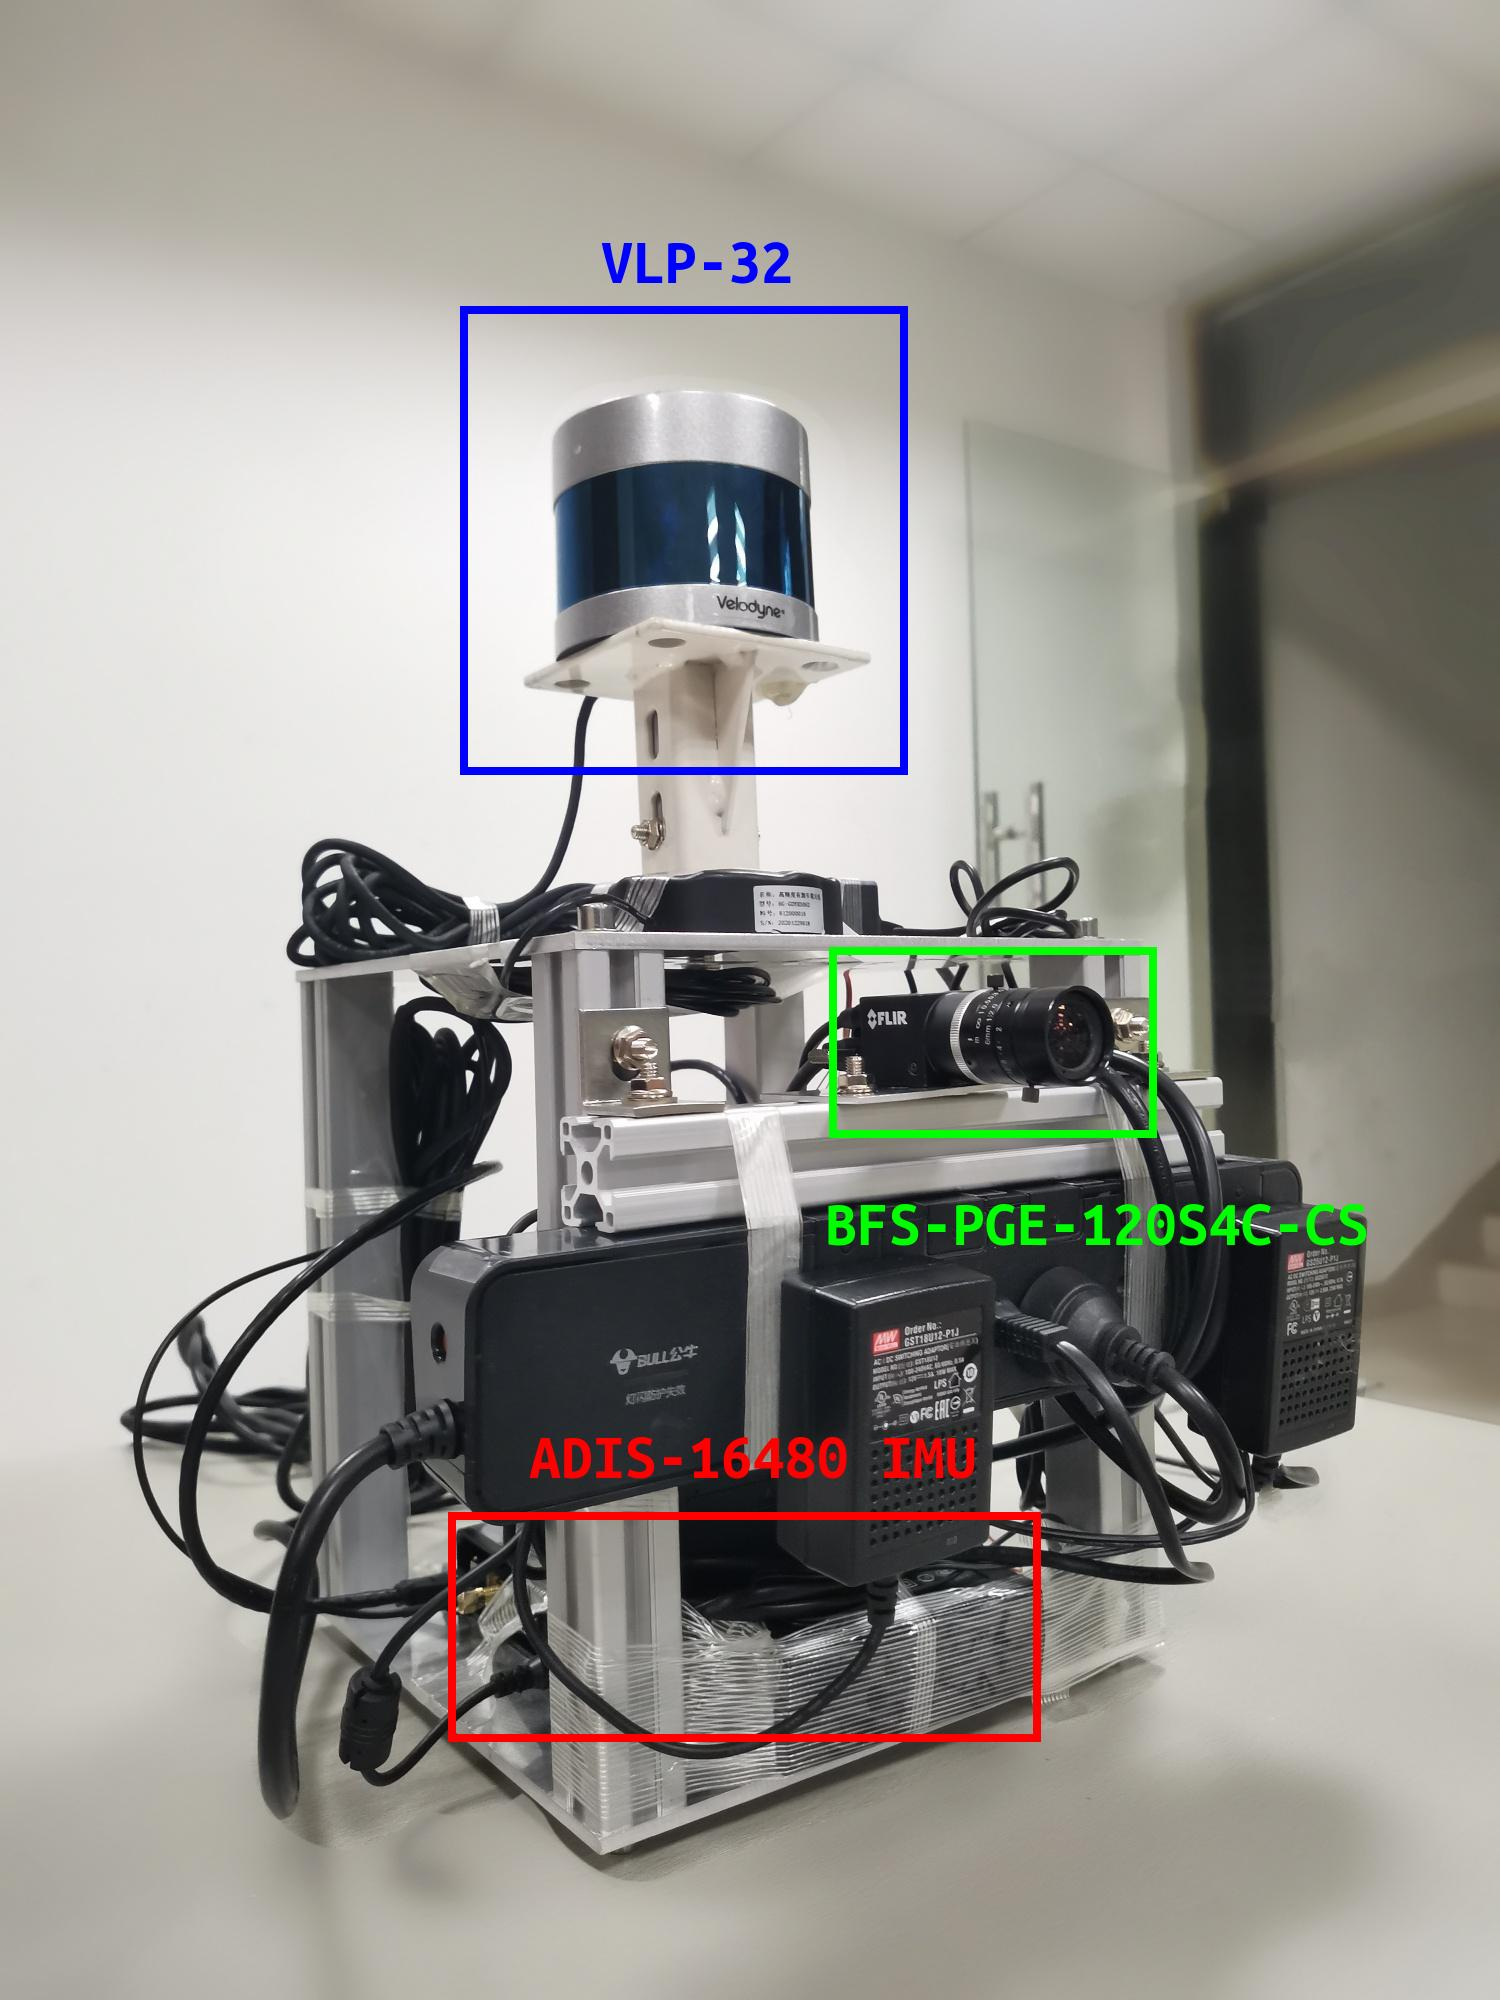
\includegraphics[width=\textwidth]{img/equipment3.jpg}}
        \vspace{20pt}
      \end{minipage}
      \label{fig:equipment}
    }
    \subfigure[\normf{实验场景:室内(上)和室外(下)}]{
      \centering
      \begin{minipage}{0.34\linewidth}
        \centerline{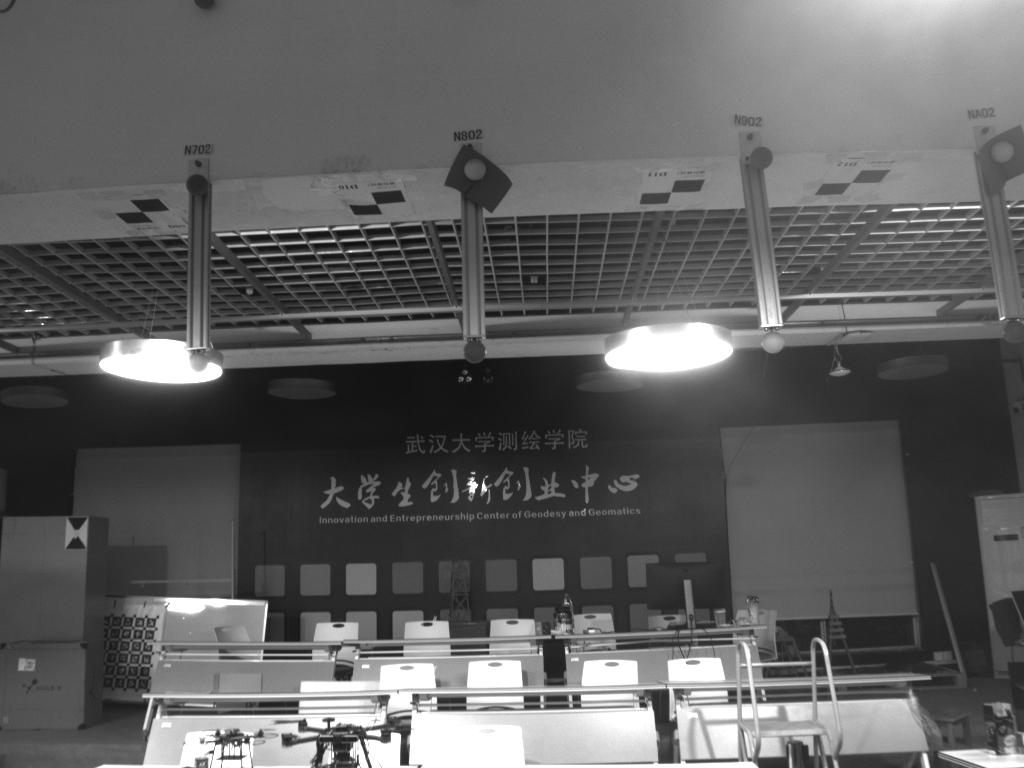
\includegraphics[width=\textwidth]{img/indoor.jpg}}
        \vspace{10pt}
        \centerline{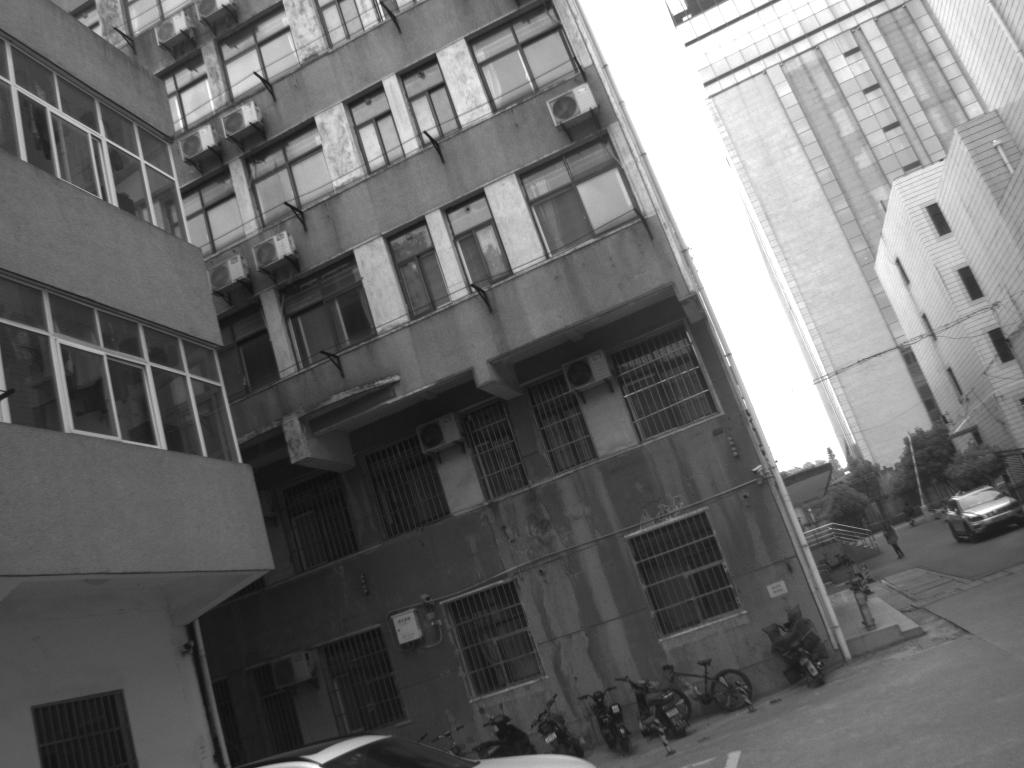
\includegraphics[width=\textwidth]{img/outdoor.jpg}}
        \vspace{20pt}
      \end{minipage}
      \label{fig:scene}
    }
    \caption{\normf{实测实验设备和场景}}
    \label{fig:simu_expr}
  \end{figure}
}
\begin{table*}[htbp]
  \centering
  \normf
  \begin{tabular}{c|ccccc}
    \hline
    {技术参数} & {线束} & {最大测距} & {测量精度} & {视场角(垂直/水平)}     & {角分辨率(垂直/水平)} \\ \hline
    {VLP-32}   & $32$   & $200\;m$   & $\pm5\;cm$ & $+15.0°\sim-25.0°/360°$ & $0.33°/0.1°\sim0.4°$  \\
    \hline
  \end{tabular}
  \caption{\normf{Velodyne VLP-32基本参数}}
  \label{tab:vlp32}
\end{table*}
\begin{table*}[htbp]
  \centering
  \normf
  \begin{tabular}{c|cccc}
    \hline
    {技术参数}             & {快门类型}            & {像素大小} & {图像尺寸} & {最高帧频} \\ \hline
    {BFS-PGE-120S4C-CS}    &
    Rolling                & $
    1.85\times1.85\;\mu m$ & $1024\times768${像素} & 30HZ                                 \\ 	\hline
  \end{tabular}
  \caption{\normf{BFS-PGE-120S4C-CS基本参数}}
  \label{tab:camera}
\end{table*}
\begin{table*}[htbp]
  \centering
  \normf
  \begin{tabular}{c|cccc}
    \hline
    {技术参数}   & {陀螺仪零偏} & {加速度计零偏} & {速度随机游走}       & {角度随机游走}    \\ \hline
    {ADIS-16480} & $8\;°/h$     & $1500\;mGal$   & $0.18\;m/s/\sqrt{h}$ & $0.3\;°/\sqrt{h}$ \\ 	\hline
  \end{tabular}
  \caption{\normf{ADIS-16480 IMU基本参数}}
  \label{tab:imu}
\end{table*}

\subsection{\normf{室内外典型场景下的算法测试和评估}}
为了让实验更具代表性,本文分别选取了室内外两个典型场景进行了标定实验,如图\ref{fig:scene}所示。在数据采集过程中,LiDAR、Camera和IMU的采样频率分别设置为10HZ、10HZ和400HZ。对于室内和室外场景下的标定解算,我们均使用了$25\;s$的数据序列,标定结果如图\ref{fig:real_world_result}所示。
%%%%%%%%%%%%%%%%%%%%%%%%%%%%%%%%%%%%%%%%%%%%%%%%%%%%%%%%%%%%%%%%%%%%%%%%%%%%%%%%%%%%%%%%%
\mlcomment{
  \begin{figure}[h]
    \centering

    \subfigure[\normf{室内}]{
      \centering
      \begin{minipage}{0.37\linewidth}
        \centerline{\includegraphics[width=\textwidth]{img/real_world/indoor/map.png}}
        \vspace{10pt}
        \centerline{\includegraphics[width=\textwidth]{img/real_world/indoor/plane.png}}
        \vspace{20pt}
      \end{minipage}
      \label{fig:scene_indoor}
    }
    \subfigure[\normf{室外}]{
      \centering
      \begin{minipage}{0.37\linewidth}
        \centerline{\includegraphics[width=\textwidth]{img/real_world/outdoor/map.png}}
        \vspace{10pt}
        \centerline{\includegraphics[width=\textwidth]{img/real_world/outdoor/plane.png}}
        \vspace{20pt}
      \end{minipage}
      \label{fig:scene_outdoor}
    }
    \subfigure[\normf{标定结果可视化}]{
      \centering
      \begin{minipage}{0.184\linewidth}
        \centerline{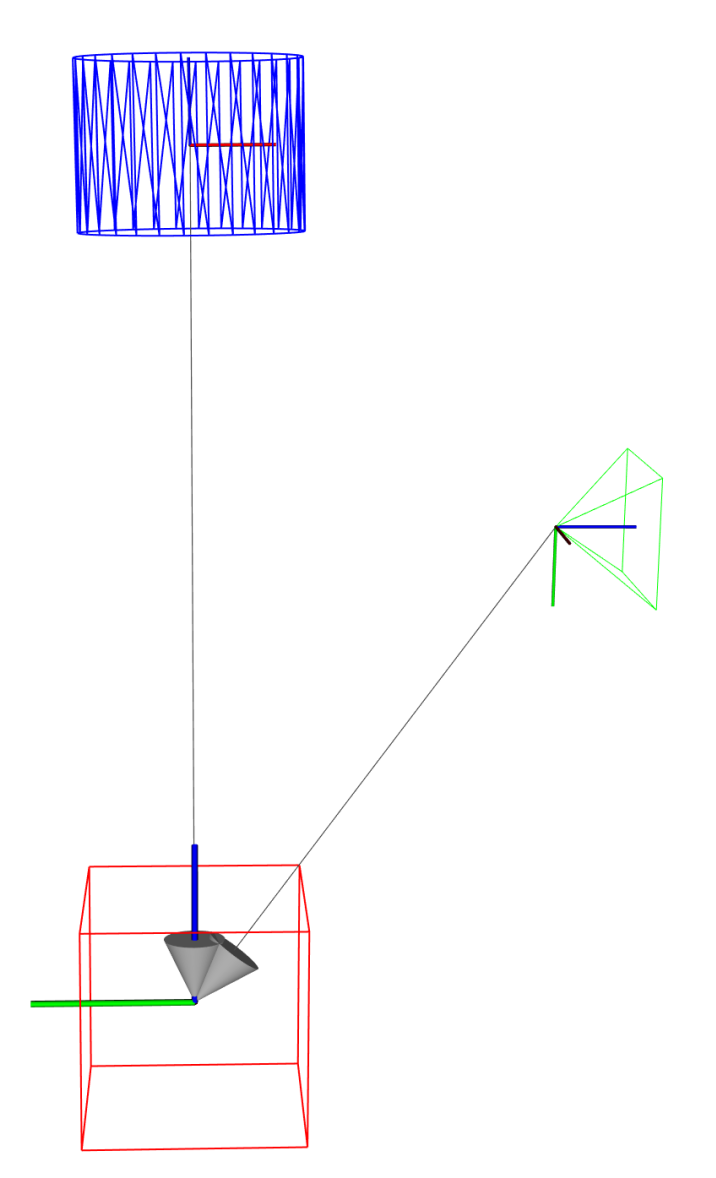
\includegraphics[width=\textwidth]{img/real_world/sensors1.png}}
        \vspace{10pt}
        \centerline{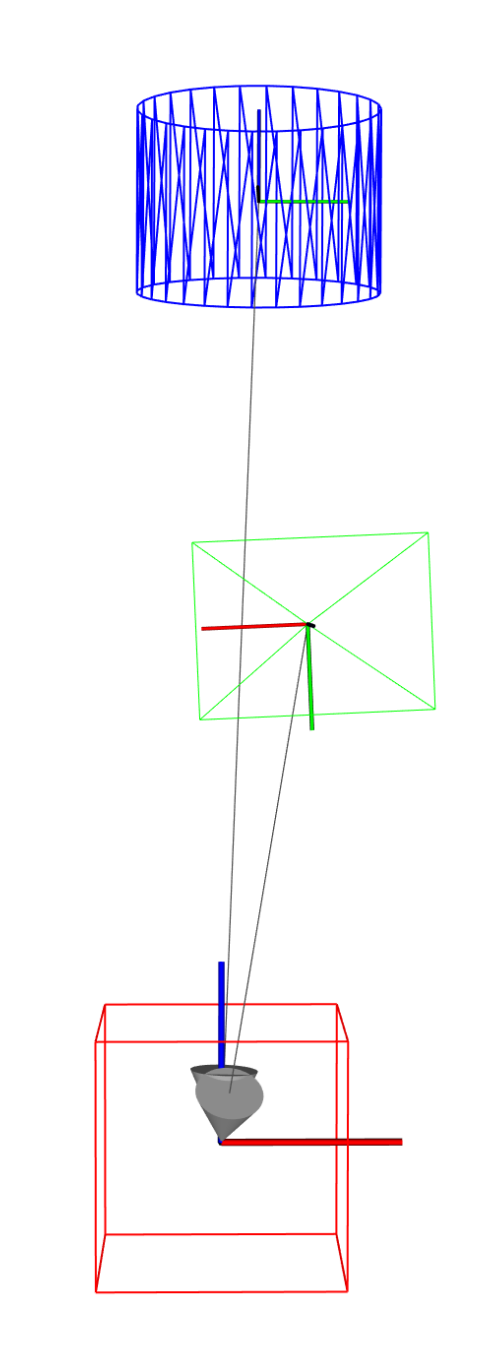
\includegraphics[width=\textwidth]{img/real_world/sensors2.png}}
        \vspace{20pt}
      \end{minipage}
      \label{fig:sensors}
    }
    \caption{\normf{实测实验解算结果}}
    \label{fig:real_world_result}
  \end{figure}
}

在实际进行解算的时候,为了保证迭代优化解算时的可靠性,避免系统陷入局部最优,我们使用了如下所述的优化策略:在首次批处理优化中,我们选择优化位姿B样条曲线和外参,同时考虑到相机尺度因子可能受到不准确相机位姿序列的影响而造成初始化不精确,该参数也会被加入到图中进行优化。其他参数在首次批处理中被固定,不进行优化。在之后的批处理优化中,我们会依次将相机内参、IMU内参加入到优化图中。最后,我们会加入时延参数进行优化,因为时参的估计易受其他未校准参数的影响。注意到,IMU位姿B样条曲线在所有的批处理中均被加入到图中优化,以为下一次的数据关联提供更为精确的先验信息。正如\ref{subsec:alg_define}节所述,我们在批处理中引入了优化选项,可以在不影响参数可观性的前提下,选择性的标定部分参数,因此上述的优化策略是易于实现的。

%%%%%%%%%%%%%%%%%%%%%%%%%%%%%%%%%%%%%%%%%%%%%%%%%%%%%%%%%%%%%%%%%%%%%%%%%%%%%%%%%%%%%%%%%
\mlcomment{
  \begin{figure}[htbp]
    \centering
    \includegraphics[width=0.95\linewidth]{img/real_world/indoor/params_iter/abs_error.png}

    \caption{\normf{室内实测实验IMU/LiDAR/Camera外参和时延的收敛曲线}}

    \label{fig:indoor_evaluate}
  \end{figure}
}
%%%%%%%%%%%%%%%%%%%%%%%%%%%%%%%%%%%%%%%%%%%%%%%%%%%%%%%%%%%%%%%%%%%%%%%%%%%%%%%%%%%%%%%%%
\mlcomment{
  \begin{figure}[htbp]
    \centering
    \includegraphics[width=0.95\linewidth]{img/real_world/outdoor/params_iter/abs_error.png}

    \caption{\normf{室外实测实验IMU/LiDAR/Camera外参和时延的收敛曲线}}

    \label{fig:outdoor_evaluate}
  \end{figure}
}
% Please add the following required packages to your document preamble:
% \usepackage{multirow}
\begin{table}[]
  \centering
  \normf
  \begin{tabular}{c|c|ccccccc}
    \hline
    \multirow{2}{*}{场景} & \multirow{2}{*}{参数} & \multicolumn{3}{c|}{外参姿态误差$(^\circ)$} & \multicolumn{3}{c|}{外参位移误差$(mm)$} & 时延$(ms)$                                                                                                                                                                    \\ \cline{3-9}
                          &                       & $\delta{\boldsymbol{\theta}(r)}$            & $\delta{\boldsymbol{\theta}(p)}$        & \multicolumn{1}{c|}{$\delta{\boldsymbol{\theta}(y)}$} & $\delta{\boldsymbol{p}(x)}$ & $\delta{\boldsymbol{p}(y)}$ & \multicolumn{1}{c|}{$\delta{\boldsymbol{p}(z)}$} & $ t$   \\ \hline
    \multirow{2}{*}{室内} & IMU/LiDAR             & 0.012                                       & 0.005                                   & 0.044                                                 & 0.374                       & 1.868                       & 0.964                                            & 5.822  \\
                          & IMU/Camera            & 0.089                                       & 0.049                                   & 0.009                                                 & 1.596                       & 2.237                       & 2.207                                            & 12.928 \\ \hline
    \multirow{2}{*}{室外} & IMU/LiDAR             & 0.034                                       & 0.043                                   & 0.015                                                 & 1.646                       & 1.862                       & 2.314                                            & 5.734  \\
                          & IMU/Camera            & 0.064                                       & 0.006                                   & 0.030                                                 & 4.774                       & 0.888                       & 4.867                                            & 6.476  \\ \hline
  \end{tabular}
  \caption{\normf{实测实验外参标定误差及时延估值}}
  \label{tab:real_world_statistic}
\end{table}

与仿真实验类似,我们对室内外实验标定过程中不同迭代次数下的外参和时延的估值进行了统计,并绘制了相应的绝对误差曲线,结果如图\ref{fig:indoor_evaluate}、\ref{fig:outdoor_evaluate}所示,图中横、纵坐标的含义与仿真实验一致。由于无法获得时延参数的真值,因此我们绘制了其状态变化曲线。可以看到,无论是室内环境还是室外环境,基于手眼标定法初始化的IMU/LiDAR和IMU/Camera外参的精度能够得到保证,尤其是IMU/Camera外参姿态量,其初始化后的偏差比IMU/LiDAR外参姿态量的初始化偏差小很多,这离不开SfM算法的鲁棒性。同时,相较于仿真实验,实测实验在前20次迭代计算中参数的波动更小,收敛特性更好。原因在于,在实测实验数据采集时我们充分激励载体运动,同时在解算时使用了更长时间的数据序列,二者对于标定问题的解算都是有利的。在算法收敛时,外参姿态量的偏差在$0.1^\circ$以内,位移量偏差在$5\;mm$以内,如表\ref{tab:real_world_statistic}所示。

同时注意到,相比与IMU/LiDAR参数的估计迭代过程,IMU/Camera相关参数在迭代过程中波动更大。原因在于,为了对SfM算法估计的场景结构进行精化,在迭代过程中我们将特征点逆深度参数向量加入到优化图中,高维数的逆深度参数向量会让图优化问题中的非线性特性变得更加严重,导致迭代求解不稳定。好在通过多次迭代线性化操作后,参数最后都会收敛到一个较优的值。
另外我们注意到,在室内、室外不同环境下,IMU/Camera的时延参数收敛值不一样:在室内环境下,相机相对于IMU的时延${^I}t_C$的估值为$12.928\;ms$,而在室外环境下,该时延参数估值为$6.476\;ms$。原因在于相较于光线充足的室外环境,室内环境光线不足,相机需要更长的曝光时间。

为了考察室内外场景下算法的收敛特征,我们对批处理优化过程中的目标函数、梯度和置信半径进行统计,并绘制了如图\ref{fig:real_world_iter_info}所示的变化曲线\footnote{\normf{图中目标函数和梯度的变化曲线已通过$\log_{10}(\cdot)$函数映射。}},其中:
\begin{enumerate}
  \item 目标函数变化曲线

        该表征了优化过程中的损失变化和收敛速度,算法损失下降越快,相应的收敛速度就越快。从图中可以看出,无论是室内场景还是室外场景,算法收敛速度较快,目标函数都能在第一次批处理优化后(BO 1)达到较小的值。

  \item 梯度变化曲线

        该曲线与优化过程中算法逼近最优解的表现相关,算法越逼近最优解,梯度越小。需要注意的是,算法无论逼近的是局部最优解还是全局最优解,对应的梯度都小。由于在每次批处理优化后都会重新进行数据关联,因此图中相邻批处理优化之间的梯度存在跳跃。从图中可以看到,每次批处理优化结束时的梯度都较小,结合目标函数变化曲线,可以说明算法能够求解得到全局最优解。

  \item 置信半径变化曲线

        由于本文使用LM法进行优化,因此我们绘制了置信半径变化曲线。置信半径$1/\lambda$
        的大小体现了LM法在迭代求解时的“自信度”,具体表现在参数更新步长方面,具体参考附录\ref{appendix:lm_alg}。从图中可以看出,由于每次批处理优化的目标函数均在减小,因此置信半径在不断增大。
\end{enumerate}
%%%%%%%%%%%%%%%%%%%%%%%%%%%%%%%%%%%%%%%%%%%%%%%%%%%%%%%%%%%%%%%%%%%%%%%%%%%%%%%%%%%%%%%%%
\mlcomment{
  \begin{figure}[htbp]
    \centering
    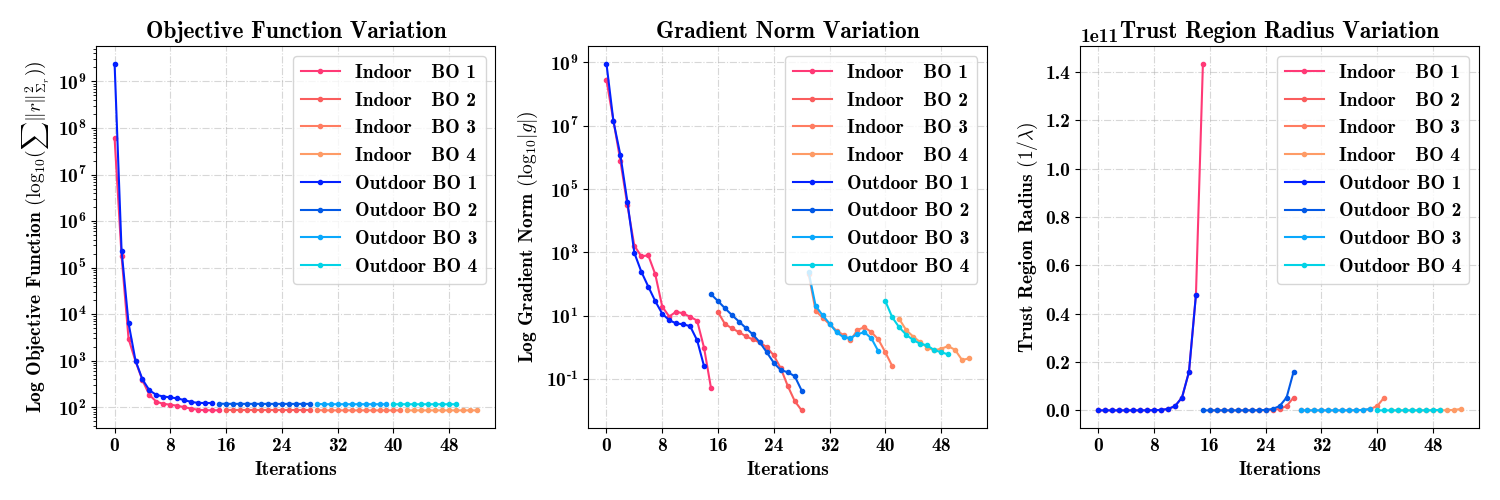
\includegraphics[width=0.95\linewidth]{img/real_world/iter_info.png}

    \caption{\normf{实测实验批处理优化中的目标函数(左)、梯度(中)和置信半径(右)变化曲线}}

    \label{fig:real_world_iter_info}
  \end{figure}
}

为了考察约束构建准确性和有效性,我们对每次批处理优化时的残差进行统计,并绘制了如图\ref{fig:real_world_residuals}所示的残差分布图。在批处理涉及的三种约束中,点到面约束和IMU/LiDAR相关参数有关,重投影约束和IMU/Camera相关参数有关,因此在分析过程中主要考虑了这两种约束对应的残差分布。从图中可以看到,无论是室内场景还是室外场景,点到面残差和重投影残差呈现零均值正态分布,并且随着批处理优化次数的增加,标准差更小,这说明了约束构建的正确性和批处理优化的有效性。同时可以发现,在第一次批处理优化后,构建的点到面约束明显增加,原因在于经过该次批处理优化,IMU/LiDAR外参中的位移量被估计,能够更好的去除点云帧中的运动畸变,从而找到更多的面特征,以构建更多、更强的点到面约束。

\mlcomment{
  \begin{figure}[htbp]
    \centering

    \subfigure[\normf{室内实验}]{
      \centering
      \includegraphics[width=0.95\linewidth]{img/real_world/indoor/residuals.png}
    }
    \subfigure[\normf{室外实验}]{
      \centering
      \includegraphics[width=0.95\linewidth]{img/real_world/outdoor/residuals.png}
    }

    \caption{\normf{批处理优化过程中的点到面残差和重投影残差分布}}

    \label{fig:real_world_residuals}
  \end{figure}
}

\subsection{\normf{算法一致性评价}}
为了更为直观的评价算法的一致性,我们基于解算完成后的IMU位姿B样条曲线$\mathcal{B}$、LiDAR点云地图$\mathcal{M}$和相机图像序列$\mathcal{C}_{\mathcal{I}}$,将灰度信息映射到点云地图上,得到了如图\ref{fig:indoor_pointcloud}、图\ref{fig:outdoor_pointcloud}所示的重建场景$\mathcal{M}^\prime$。结果点云地图$\mathcal{M}^\prime$相较于原始输入的LiDAR点云地图$\mathcal{M}$,附带有灰度信息。因此,通过$\mathcal{M}^\prime$能够比较直观的查看地图几何结构和灰度属性之间的对应关系,从而对算法的一致性进行评价。具体来说,对于点$\boldsymbol{p}\in\mathcal{M}$,查询能够正常观察到该点的图像序列,并通过采样构造灰度向量。为了让场景亮度具有一致性,我们将该灰度向量的均值作为该点的灰度,处理流程如算法\ref{alg:color_map}所示。
\begin{algorithm}[htbp]
  \label{alg:color_map}
  \caption{\normf{构建带有灰度纹理的三维场景}}
  \LinesNumbered 
  \KwIn{\normf{IMU位姿B样条曲线$\mathcal{B}$、LiDAR点云地图$\mathcal{M}$和相机图像序列$\mathcal{C}_{\mathcal{I}}$}}%输入参数
  \KwOut{\normf{带有灰度纹理的三维场景$\mathcal{M}^\prime$}}
  \ForEach{$\boldsymbol{p}\in\mathcal{M}$}{
    \normf{初始化灰度集合:}$\mathcal{G}_{\boldsymbol{p}}=\left\lbrace \right\rbrace $\;
    \ForEach{$i\in\left( \mathcal{C}_{\mathcal{I}}\right) ^\dagger$}{
      \normf{将点变换到第$i$个相机坐标系下:}
      $\boldsymbol{p}^\prime\gets\begin{pmatrix}
      \boldsymbol{p}^\prime\\1			\end{pmatrix}={{^{I}_{C}}\boldsymbol{T}^{-1}}\cdot{{^{I_0}_{I}}\boldsymbol{T}^{-1}\left( t_{C_i}+{^{I}t_C}\right) }\cdot{{^{I_0}_{I}}\boldsymbol{T}\left( t_{L}(\boldsymbol{p})+{^{I}t_L}\right) }\cdot{{^{I}_{L}}\boldsymbol{T}}\begin{pmatrix}
      \boldsymbol{p}\\1
      \end{pmatrix}$\;
      
      \If{$\boldsymbol{p}^\prime_z>0\;\boldsymbol{\&}\;\pi(\boldsymbol{p}^\prime)\in\mathcal{C}_{\mathcal{I}_i}$}{
        \normf{记录能被正常观测得到的点的灰度:}
        $\mathcal{G}_{\boldsymbol{p}}\gets\mathcal{C}_{\mathcal{I}_i}\left( \pi(\boldsymbol{p}^\prime)\right) $\;
      }
    }
    \If{$\mathcal{G}_{\boldsymbol{p}}\neq\boldsymbol{\varnothing}$}{
      $c=0,\;g_s=0$\;
      \ForEach{$g\in\mathcal{G}_{\boldsymbol{p}}$}{
        $g_s=g_s+g,\;c=c+1$\;
      }
      \normf{记录点及其灰度均值:}
      $\mathcal{M}^\prime\gets\left\lbrace \boldsymbol{p}\mid g_s/c\right\rbrace $\;
    }
  }	
\end{algorithm}

反过来,我们通过类似的处理,将点云投射到影像上,结果如图\ref{fig:indoor_view}、图\ref{fig:outdoor_view}所示,图中不同颜色代表不同深度。从图\ref{fig:pointcloud}中可以看到,无论是室内场景还是室外场景,重建的结果都有较高的一致性,主要体现在:
\begin{enumerate}
  \item 重建的点云地图结构和灰度地图一致。在灰度映射的点云地图中,几何结构和灰度信息对应得较好,如室内场景中标牌上的文字能够被清晰的重建出来。
  
  \item 重建的点云地图相对结构一致。如室外场景中位于过道上的门窗排列一致,过道前不同停车位之间的几何连接是一致的。
  
  \item “深度”影像的物体和原始影像上同名物体之间的几何位置对应得很好。
\end{enumerate}

综上可见,本文所提出的基于连续时间的LiDAR/Camera/IMU的时空标定方法能够在保证整个标定系统一致的条件下,求得全局最优的解。

%%%%%%%%%%%%%%%%%%%%%%%%%%%%%%%%%%%%%%%%%%%%%%%%%%%%%%%%%%%%%%%%%%%%%%%%%%%%%%%%%%%%%%%%%
\mlcomment{	
\begin{figure}[htbp]
  \centering
    \subfigure[\normf{室内上色点云地图}]{
  \centering
    \includegraphics[width=0.4\linewidth]{img/real_world/indoor/pointcloud1.png}
    \includegraphics[width=0.4\linewidth]{img/real_world/indoor/pointcloud2.png}
  \label{fig:indoor_pointcloud}
  }
  \subfigure[\normf{室内共视视角}]{
    \centering
    \includegraphics[width=0.2\linewidth]{img/real_world/indoor/image_view1.png}
    \includegraphics[width=0.2\linewidth]{img/real_world/indoor/map_view1.png}
    \includegraphics[width=0.2\linewidth]{img/real_world/indoor/image_view2.png}
    \includegraphics[width=0.2\linewidth]{img/real_world/indoor/map_view2.png}
    \label{fig:indoor_view}
  }
  \subfigure[\normf{室外上色点云地图}]{
    \centering
    \includegraphics[width=0.4\linewidth]{img/real_world/outdoor/pointcloud1.png}
    \includegraphics[width=0.4\linewidth]{img/real_world/outdoor/pointcloud2.png}
    \label{fig:outdoor_pointcloud}
  }
        \subfigure[\normf{室外共视视角}]{
    \centering
    \includegraphics[width=0.2\linewidth]{img/real_world/outdoor/image_view1.png}
    \includegraphics[width=0.2\linewidth]{img/real_world/outdoor/map_view1.png}
    \includegraphics[width=0.2\linewidth]{img/real_world/outdoor/image_view2.png}
    \includegraphics[width=0.2\linewidth]{img/real_world/outdoor/map_view2.png}
    \label{fig:outdoor_view}
  }
  \caption{\normf{实测实验场景重建}}
  
  \label{fig:pointcloud}
\end{figure}
}

\section{\normf{系统可观性实验}}
\label{appendix:observability}
系统的可观性是指基于系统的有限输入和输出信息,能否唯一确定系统在某个时刻的状态信息的性质\cite{bubnicki2005modern}。当系统的状态能够被完全确定时,称系统可观;当系统的部分状态可以被确定时,称系统部分可观;当系统的状态都不能确定时,称系统不可观。由于本文提出的基于连续时间的LiDAR/Camera/IMU的时空标定方法是一种通过自运动估计的无靶标标定方法,在标定的过程中需要充分的运动激励来保证系统的可观性。如果在标定时载体的运动不充分,会严重损害估计参数的精度,甚至导致参数不可观,无法被估计出来。为此,有必要对系统在不同运动形式下的可观性进行分析和测试。

\subsection{\normf{基于法方程的系统可观性分析}}
如前文所述,本文提出的标定系统是一个基于图优化的标定框架,因此不能像滤波优化方法\cite{huai2022observability}、\cite{mirzaei2008kalman}、\cite{yang2019degenerate}、\cite{lv2022observability}一样,通过能观性秩条件(Observability Rank Condition,ORC)对系统的可观性进行判定。
与滤波优化方法不同,图优化方法在每次迭代中,基于高斯牛顿法或者LM法(本文使用LM法,算法细节见附录\ref{appendix:lm_alg})构建法方程,而后求解该方程并对参数进行增量更新。因此,本文从法方程的角度出发进行系统的可观性分析。在不考虑置信域的情况下,LM方法的法方程如下所示:
\begin{equation}
  \boldsymbol{H}_{n\times n}\cdot\delta\boldsymbol{x}_{n\times 1}=\boldsymbol{b}_{n\times 1}
  \quad
  \mathrm{s.t.}
  \quad
  \begin{cases}
    \begin{aligned}
      \boldsymbol{H}_{n\times n} & =	\left( \frac{\partial^2 \boldsymbol{r}(\boldsymbol{x})}{\partial \boldsymbol{x}^T}\bigg|_{\boldsymbol{x}_{op}}\right)^T
      \left( \frac{\partial^2 \boldsymbol{r}(\boldsymbol{x})}{\partial \boldsymbol{x}}\bigg|_{\boldsymbol{x}_{op}}\right)                                                                       \\
      \boldsymbol{b}_{n\times 1} & =-\left( \frac{\partial^2 \boldsymbol{r}(\boldsymbol{x})}{\partial \boldsymbol{x}^T}\bigg|_{\boldsymbol{x}_{op}}\right)^T\boldsymbol{r}(\boldsymbol{x}_{op})
    \end{aligned}
  \end{cases}
\end{equation}
其中:$\delta\boldsymbol{x}_{n\times1}$为的参数更新向量;$\boldsymbol{x}_{op}$为参数向量的优化初值;$\boldsymbol{r}(\boldsymbol{x})$为损失函数。
为了简洁,对于参数更新向量$\delta\boldsymbol{x}$,我们只考虑系统的外参和时延参数,不考虑其余参数:
\begin{equation}
  \begin{aligned}
    \delta\boldsymbol{x}      & =\left\lbrace
    \delta\boldsymbol{x}_{ex},\delta\boldsymbol{x}_{t}
    \right\rbrace_{14\times 1}                                                                                                                                                                                \\
    \delta\boldsymbol{x}_{ex} & =\left\lbrace \delta{^{I}_{L}\boldsymbol{\theta}},\delta{^{I}}\boldsymbol{p}_{L},\delta{^{I}_{C}\boldsymbol{\theta}},\delta{^{I}}\boldsymbol{p}_{C}\right\rbrace_{12\times 1} \\
    \delta\boldsymbol{x}_{t}  & =\left\lbrace \delta{^{I}t_{L}},\delta{^{I}t_{C}}\right\rbrace_{2\times 1}                                                                                                    \\
  \end{aligned}
\end{equation}
另外,在\ref{sect:batch_optimization}节中批处理优化时涉及的四种因子中,点到面因子与LiDAR的外参和时参求解相关,重投影因子与Camera的外参和时参求解相关,因此令残差向量为:
\begin{equation}
  \boldsymbol{r}_{3\times 1}=\begin{pmatrix}
    \boldsymbol{r}_{ij}^k(l) \\\boldsymbol{r}_{ij}^{mn}(c)
  \end{pmatrix}
  \simeq
  \begin{pmatrix}
    \boldsymbol{r}(l) \\\boldsymbol{r}(c)
  \end{pmatrix}
\end{equation}
则残差$\boldsymbol{r}$对参数$\delta\boldsymbol{x}$的雅克比矩阵为:
\begin{equation}
  \boldsymbol{J}_{\boldsymbol{x}}=\frac{\partial \boldsymbol{r}}{\partial \delta \boldsymbol{x}}=
  \begin{pmatrix}
    \frac{\partial \boldsymbol{r}(l)}{\partial \delta {^{I}_{L}\boldsymbol{\theta}}} &
    \frac{\partial \boldsymbol{r}(l)}{\partial \delta {^{I}\boldsymbol{p}_L}}        &
    \boldsymbol{0}_{1\times 3}                                                       &
    \boldsymbol{0}_{1\times 3}                                                       &
    \frac{\partial \boldsymbol{r}(l)}{\partial \delta {^{I}t_{L}}}                   &
    \boldsymbol{0}_{1\times 1}                                                         \\
    \boldsymbol{0}_{2\times 3}                                                       &
    \boldsymbol{0}_{2\times 3}                                                       &
    \frac{\partial \boldsymbol{r}(c)}{\partial \delta {^{I}_{C}\boldsymbol{\theta}}} &
    \frac{\partial \boldsymbol{r}(c)}{\partial \delta {^{I}\boldsymbol{p}_C}}        &
    \boldsymbol{0}_{2\times 1}                                                       &
    \frac{\partial \boldsymbol{r}(c)}{\partial \delta {^{I}t_{C}}}
  \end{pmatrix}_{3\times 14}
\end{equation}
每次迭代更新构建的法方程为:
\begin{equation}
  \underbrace{\left(
    \sum\boldsymbol{J}_{\boldsymbol{x}}^T\cdot\boldsymbol{J}_{\boldsymbol{x}}
    \right)}_{\boldsymbol{H}_{14\times 14}}
  \cdot\delta\boldsymbol{x}=
  \underbrace{\left( -\sum \boldsymbol{J}_{\boldsymbol{x}}^T\cdot\boldsymbol{r}\right)}
  _{\boldsymbol{b}_{14\times 1}}\to\boldsymbol{H}
  \cdot\delta\boldsymbol{x}=\boldsymbol{b}
\end{equation}
其中系数矩阵$\boldsymbol{H}$为:
\begin{equation*}
  \sum\begin{pmatrix}
    \frac{\partial \boldsymbol{r}(l)}{\partial \delta {^{I}_{L}\boldsymbol{\theta}}}^T
    \cdot \frac{\partial \boldsymbol{r}(l)}{\partial \delta {^{I}_{L}\boldsymbol{\theta}}} &
    \frac{\partial \boldsymbol{r}(l)}{\partial \delta {^{I}_{L}\boldsymbol{\theta}}}^T
    \cdot \frac{\partial \boldsymbol{r}(l)}{\partial \delta {^{I}\boldsymbol{p}_L}}        &
    \boldsymbol{0}_{3\times 3}                                                             &
    \boldsymbol{0}_{3\times 3}                                                             &
    \frac{\partial \boldsymbol{r}(l)}{\partial \delta {^{I}_{L}\boldsymbol{\theta}}}^T
    \cdot \frac{\partial \boldsymbol{r}(l)}{\partial \delta {^{I}t_{L}}}                   &
    \boldsymbol{0}_{3\times 1}                                                               \\
    \frac{\partial \boldsymbol{r}(l)}{\partial \delta {^{I}\boldsymbol{p}_L}}^T
    \cdot \frac{\partial \boldsymbol{r}(l)}{\partial \delta {^{I}_{L}\boldsymbol{\theta}}} &
    \frac{\partial \boldsymbol{r}(l)}{\partial \delta {^{I}\boldsymbol{p}_L}}^T
    \cdot \frac{\partial \boldsymbol{r}(l)}{\partial \delta {^{I}\boldsymbol{p}_L}}        &
    \boldsymbol{0}_{3\times 3}                                                             &
    \boldsymbol{0}_{3\times 3}                                                             &
    \frac{\partial \boldsymbol{r}(l)}{\partial \delta {^{I}\boldsymbol{p}_L}}^T
    \cdot \frac{\partial \boldsymbol{r}(l)}{\partial \delta {^{I}t_{L}}}                   &
    \boldsymbol{0}_{3\times 1}                                                               \\
    \boldsymbol{0}_{3\times 3}                                                             &
    \boldsymbol{0}_{3\times 3}                                                             &
    \frac{\partial \boldsymbol{r}(c)}{\partial \delta {^{I}_{C}\boldsymbol{\theta}}}^T
    \cdot \frac{\partial \boldsymbol{r}(c)}{\partial \delta {^{I}_{C}\boldsymbol{\theta}}} &
    \frac{\partial \boldsymbol{r}(c)}{\partial \delta {^{I}_{C}\boldsymbol{\theta}}}^T
    \cdot \frac{\partial \boldsymbol{r}(c)}{\partial \delta {^{I}\boldsymbol{p}_C}}        &
    \boldsymbol{0}_{3\times 1}                                                             &
    \frac{\partial \boldsymbol{r}(c)}{\partial \delta {^{I}_{C}\boldsymbol{\theta}}}^T
    \cdot \frac{\partial \boldsymbol{r}(c)}{\partial \delta {^{I}t_{C}}}                     \\
    \boldsymbol{0}_{3\times 3}                                                             &
    \boldsymbol{0}_{3\times 3}                                                             &
    \frac{\partial \boldsymbol{r}(c)}{\partial \delta {^{I}\boldsymbol{p}_C}}^T
    \cdot\frac{\partial \boldsymbol{r}(c)}{\partial \delta {^{I}_{C}\boldsymbol{\theta}}}  &
    \frac{\partial \boldsymbol{r}(c)}{\partial \delta {^{I}\boldsymbol{p}_C}}^T
    \cdot\frac{\partial \boldsymbol{r}(c)}{\partial \delta {^{I}\boldsymbol{p}_C}}         &
    \boldsymbol{0}_{3\times 1}                                                             &
    \frac{\partial \boldsymbol{r}(c)}{\partial \delta {^{I}\boldsymbol{p}_C}}^T
    \cdot\frac{\partial \boldsymbol{r}(c)}{\partial \delta {^{I}t_{C}}}                      \\
    \frac{\partial \boldsymbol{r}(l)}{\partial \delta {^{I}t_{L}}}^T
    \cdot\frac{\partial \boldsymbol{r}(l)}{\partial \delta {^{I}_{L}\boldsymbol{\theta}}}  &
    \frac{\partial \boldsymbol{r}(l)}{\partial \delta {^{I}t_{L}}}^T
    \cdot\frac{\partial \boldsymbol{r}(l)}{\partial \delta {^{I}\boldsymbol{p}_L}}         &
    \boldsymbol{0}_{1\times 3}                                                             &
    \boldsymbol{0}_{1\times 3}                                                             &
    \frac{\partial \boldsymbol{r}(l)}{\partial \delta {^{I}t_{L}}}^T
    \cdot\frac{\partial \boldsymbol{r}(l)}{\partial \delta {^{I}t_{L}}}                    &
    \boldsymbol{0}_{1\times 1}                                                               \\
    \boldsymbol{0}_{1\times 3}                                                             &
    \boldsymbol{0}_{1\times 3}                                                             &
    \frac{\partial \boldsymbol{r}(c)}{\partial \delta {^{I}t_{C}}}^T
    \cdot\frac{\partial \boldsymbol{r}(c)}{\partial \delta {^{I}_{C}\boldsymbol{\theta}}}  &
    \frac{\partial \boldsymbol{r}(c)}{\partial \delta {^{I}t_{C}}}^T
    \cdot\frac{\partial \boldsymbol{r}(c)}{\partial \delta {^{I}\boldsymbol{p}_C}}         &
    \boldsymbol{0}_{1\times 1}                                                             &
    \frac{\partial \boldsymbol{r}(c)}{\partial \delta {^{I}t_{C}}}^T
    \cdot\frac{\partial \boldsymbol{r}(c)}{\partial \delta {^{I}t_{C}}}                      \\
  \end{pmatrix}
\end{equation*}
向量$\boldsymbol{b}$为:
\begin{equation*}
  \sum\begin{pmatrix}
    \frac{\partial \boldsymbol{r}(l)}{\partial \delta {^{I}_{L}\boldsymbol{\theta}}}\cdot\boldsymbol{r}^T(l) &
    \frac{\partial \boldsymbol{r}(l)}{\partial \delta {^{I}\boldsymbol{p}_L}}\cdot\boldsymbol{r}^T(l)        &
    \frac{\partial \boldsymbol{r}(c)}{\partial \delta {^{I}_{C}\boldsymbol{\theta}}}\cdot\boldsymbol{r}^T(c) &
    \frac{\partial \boldsymbol{r}(c)}{\partial \delta {^{I}\boldsymbol{p}_C}}\cdot\boldsymbol{r}^T(c)        &
    \frac{\partial \boldsymbol{r}(l)}{\partial \delta {^{I}t_{L}}}\cdot\boldsymbol{r}^T(l)                   &
    \frac{\partial \boldsymbol{r}(c)}{\partial \delta {^{I}t_{C}}}\cdot\boldsymbol{r}^T(c)
  \end{pmatrix}^T
\end{equation*}
具体的雅克比矩阵(偏导数矩阵)如附录\ref{sect:point_to_plnae_factor_jacobian}、\ref{sect:reproject_factor_jacobian}所示。

\begin{itemize}
  \item[$\blacksquare$]参数可观性判定
\end{itemize}

对于法方程$\boldsymbol{H}_{n\times n}\cdot\delta\boldsymbol{x}_{n\times 1}=\boldsymbol{b}_{n\times 1}$,记$\bar{\boldsymbol{H}}_{n\times (n+1)}=\left[\boldsymbol{H}_{n\times n}\mid \boldsymbol{b}_{n\times 1}\right]$为增广矩阵,则:
\begin{enumerate}
  \item 当$r[\boldsymbol{H}_{n\times n}]=r[\bar{\boldsymbol{H}}_{n\times (n+1)}]=n$时,方程有唯一解,此时系统完全可观,且有$\delta\boldsymbol{x}_{n\times 1}=\boldsymbol{H}^{-1}_{n\times n}\cdot\boldsymbol{b}_{n\times 1}$;

  \item 当$r[\boldsymbol{H}_{n\times n}]=r[\bar{\boldsymbol{H}}_{n\times (n+1)}]<n$时,方程有无穷多解,此时系统部分可观或完全不可观;

  \item 当$r[\boldsymbol{H}_{n\times n}]\ne r[\bar{\boldsymbol{H}}_{n\times (n+1)}]$时,方程无解,此时与系统可观性无关;
\end{enumerate}
其中$r[\cdot]$为求列秩运算。本文主要考量第一、第二种情况,即当方程存在解时,考察系统涉及参数的可观性。为此,设$N(\boldsymbol{H}_{n\times n})$为系数矩阵$\boldsymbol{H}_{n\times n}$的零空间(Null Space),$\boldsymbol{\xi}_1$、$\boldsymbol{\xi}_2$、$\cdots$、$\boldsymbol{\xi}_{n-r[\boldsymbol{H}]}$为零空间$N(\boldsymbol{H}_{n\times n})$的基向量,则有如下的齐次线性方程组成立:
\begin{equation}
  \boldsymbol{H}_{n\times n}\cdot\delta\boldsymbol{x}_{null}=\boldsymbol{0}_{n\times 1}\quad\mathrm{s.t.}\quad \delta\boldsymbol{x}_{null}=k_1\cdot\boldsymbol{\xi}_1+k_2\cdot\boldsymbol{\xi}_2+\cdots+k_m\cdot\boldsymbol{\xi}_{n-r[\boldsymbol{H}]}
\end{equation}
零空间的基向量可以通过对系数矩阵$\boldsymbol{H}_{n\times n}$进行LU分解获得。设$\delta\boldsymbol{x}_{part}$为非齐次线性方程组$\boldsymbol{H}_{n\times n}\cdot\delta\boldsymbol{x}_{n\times 1}=\boldsymbol{b}_{n\times 1}$的一个特解,则该方程组的完整解$\delta\boldsymbol{x}_{comp}$可以表示为特解$\delta\boldsymbol{x}_{part}$和零空间内向量$\delta\boldsymbol{x}_{null}$的线性组合(见附录\ref{sect:null_space}):
\begin{equation}
  \delta\boldsymbol{x}_{comp}=\delta\boldsymbol{x}_{part}+\delta\boldsymbol{x}_{null}=\delta\boldsymbol{x}_{part}+k_1\cdot\boldsymbol{\xi}_1+k_2\cdot\boldsymbol{\xi}_2+\cdots+k_m\cdot\boldsymbol{\xi}_{n-r[\boldsymbol{H}]}
\end{equation}
显然,当$\delta\boldsymbol{x}_{null}
  \equiv\boldsymbol{0}_{n\times 1}$时,非齐次线性方程组有唯一解。同理,对于第$i\in\left\lbrace 1,\cdots,n\right\rbrace $个待求参数$\delta\boldsymbol{x}(i)$,通过考察$\delta\boldsymbol{x}_{null}$的第$i$个元素$\delta\boldsymbol{x}_{null}(i)$来进行参数解情况的判定:
\begin{equation}
  \begin{cases}
    \delta\boldsymbol{x}_{null}(i)\equiv 0\to \delta\boldsymbol{x}_{comp}(i)\equiv\delta\boldsymbol{x}_{part}(i)                              & \to\mbox{存在唯一}\;\delta\boldsymbol{x}(i) \\
    \delta\boldsymbol{x}_{null}(i)\not\equiv 0\to\delta\boldsymbol{x}_{comp}(i)=\delta\boldsymbol{x}_{part}(i)+\delta\boldsymbol{x}_{null}(i) & \to\mbox{存在多个}\;\delta\boldsymbol{x}(i)
  \end{cases}
\end{equation}
显然,当参数更新量$\delta\boldsymbol{x}(i)$唯一时,待定参数$\boldsymbol{x}(i)$在每次迭代中能被唯一确定,表示该参数可观;当更新量$\delta\boldsymbol{x}(i)$不唯一时,对应的待求参数$\boldsymbol{x}(i)$在每次迭代中不能被唯一确定,表示该参数不可观。

在对不同类型的退化运动进行系统可观性分析时,本文主要考虑了以下的五种运动:
\begin{enumerate}
  \item 无运动:载体在三维空间中处于静止状态,即有${^{I_0}\dot{\boldsymbol{p}}_{I}(t)}=\boldsymbol{0}_{3\times 1}$和${^{I_0}_{I}\dot{\boldsymbol{\phi}}(t)}=\boldsymbol{0}_{3\times 1}$;
  \item 纯位移:载体在三维空间中只存在平移,不存在旋转,即有${^{I_0}_{I}\dot{\boldsymbol{\phi}}(t)}=\boldsymbol{0}_{3\times 1}$;
  \item 单轴旋转:载体在三维空间中绕某个轴旋转,即有$\liehat{{^{I_0}_{I}{\boldsymbol{\phi}}(t_1)}}\cdot{^{I_0}_{I}{\boldsymbol{\phi}}(t_2)}=\boldsymbol{0}_{3\times 1}$;
  \item 匀速圆周运动:载体在三维空间中运动时,IMU的线速度和角速率输出恒定不变,即有${^{I}\dot{\boldsymbol{\omega}}}=\boldsymbol{0}_{3\times 1}$和${^{I}\dot{\boldsymbol{v}}}=\boldsymbol{0}_{3\times 1}$;
  \item 随机运动:载体在三维空间中自由运动;
\end{enumerate}
上述运动类型中,除了随机运动,其他的都属于退化运动(Degenerate Motion)。为了分析的方便,我们基于一组残差构建的法方程进行系统可观性分析:
\begin{equation}
  \underbrace{\left(
    \boldsymbol{J}_{\boldsymbol{x}}^T\cdot\boldsymbol{J}_{\boldsymbol{x}}
    \right)}_{\boldsymbol{H}_i}
  \cdot\delta\boldsymbol{x}=
  \underbrace{\left( - \boldsymbol{J}_{\boldsymbol{x}}^T\cdot\boldsymbol{r}\right)}
  _{\boldsymbol{b}_i}
  \quad\to\quad
  \boldsymbol{H}_i\cdot\delta\boldsymbol{x}=\boldsymbol{b}_i
\end{equation}

\begin{itemize}
  \item[$\blacksquare$]无运动
\end{itemize}

显然,此时有:
\begin{equation}
  \boldsymbol{H}_i=\boldsymbol{0}_{14\times 14}
\end{equation}
由于$n-r\left[ \boldsymbol{H}_i\right] =14$,因此矩阵$\boldsymbol{H}_i$的零空间$N(\boldsymbol{H}_i)$由14个基向量张成:
\begin{equation}
  N(\boldsymbol{H}_i)=\mathrm{span}\left\lbrace
  \boldsymbol{\xi}_1,\boldsymbol{\xi}_2,\cdots,\boldsymbol{\xi}_{14}
  \right\rbrace
  \quad\mathrm{s.t.}\quad
  \begin{pmatrix}
    \boldsymbol{\xi}_1 & \boldsymbol{\xi}_2 & \cdots & \boldsymbol{\xi}_{14}
  \end{pmatrix}=\boldsymbol{I}_{14\times 14}
\end{equation}
由于零空间$N(\boldsymbol{H}_i)$基向量任意线性组合得到的向量$\delta\boldsymbol{x}_{null}\not\equiv\boldsymbol{0}$,因此方程存在无穷多解。且零空间向量$\delta\boldsymbol{x}_{null}$每个分量均不恒为0,因此外参和时延均不可观。
\begin{itemize}
  \item[$\blacksquare$]纯位移
\end{itemize}

此时,有:
\begin{equation}
  \frac{\partial \boldsymbol{r}(l)}{\partial \delta {^{I}\boldsymbol{p}_L}}=\boldsymbol{0}_{1\times 3}
  \quad
  \frac{\partial \boldsymbol{r}(c)}{\partial \delta {^{I}\boldsymbol{p}_C}}=\boldsymbol{0}_{2\times 3}
\end{equation}
对应的系数矩阵为:
\begin{equation*}
  \boldsymbol{H}_i=\begin{pmatrix}
    \frac{\partial \boldsymbol{r}(l)}{\partial \delta {^{I}_{L}\boldsymbol{\theta}}}^T
    \cdot \frac{\partial \boldsymbol{r}(l)}{\partial \delta {^{I}_{L}\boldsymbol{\theta}}} &
    \boldsymbol{0}_{3\times 3}                                                             &
    \boldsymbol{0}_{3\times 3}                                                             &
    \boldsymbol{0}_{3\times 3}                                                             &
    \frac{\partial \boldsymbol{r}(l)}{\partial \delta {^{I}_{L}\boldsymbol{\theta}}}^T
    \cdot \frac{\partial \boldsymbol{r}(l)}{\partial \delta {^{I}t_{L}}}                   &
    \boldsymbol{0}_{3\times 1}                                                               \\
    \boldsymbol{0}_{3\times 3}                                                             &
    \boldsymbol{0}_{3\times 3}                                                             &
    \boldsymbol{0}_{3\times 3}                                                             &
    \boldsymbol{0}_{3\times 3}                                                             &
    \boldsymbol{0}_{3\times 1}                                                             &
    \boldsymbol{0}_{3\times 1}                                                               \\
    \boldsymbol{0}_{3\times 3}                                                             &
    \boldsymbol{0}_{3\times 3}                                                             &
    \frac{\partial \boldsymbol{r}(c)}{\partial \delta {^{I}_{C}\boldsymbol{\theta}}}^T
    \cdot \frac{\partial \boldsymbol{r}(c)}{\partial \delta {^{I}_{C}\boldsymbol{\theta}}} &
    \boldsymbol{0}_{3\times 3}                                                             &
    \boldsymbol{0}_{3\times 1}                                                             &
    \frac{\partial \boldsymbol{r}(c)}{\partial \delta {^{I}_{C}\boldsymbol{\theta}}}^T
    \cdot \frac{\partial \boldsymbol{r}(c)}{\partial \delta {^{I}t_{C}}}                     \\
    \boldsymbol{0}_{3\times 3}                                                             &
    \boldsymbol{0}_{3\times 3}                                                             &
    \boldsymbol{0}_{3\times 3}                                                             &
    \boldsymbol{0}_{3\times 3}                                                             &
    \boldsymbol{0}_{3\times 1}                                                             &
    \boldsymbol{0}_{3\times 1}                                                               \\
    \frac{\partial \boldsymbol{r}(l)}{\partial \delta {^{I}t_{L}}}^T
    \cdot\frac{\partial \boldsymbol{r}(l)}{\partial \delta {^{I}_{L}\boldsymbol{\theta}}}  &
    \boldsymbol{0}_{1\times 3}                                                             &
    \boldsymbol{0}_{1\times 3}                                                             &
    \boldsymbol{0}_{1\times 3}                                                             &
    \frac{\partial \boldsymbol{r}(l)}{\partial \delta {^{I}t_{L}}}^T
    \cdot\frac{\partial \boldsymbol{r}(l)}{\partial \delta {^{I}t_{L}}}                    &
    \boldsymbol{0}_{1\times 1}                                                               \\
    \boldsymbol{0}_{1\times 3}                                                             &
    \boldsymbol{0}_{1\times 3}                                                             &
    \frac{\partial \boldsymbol{r}(c)}{\partial \delta {^{I}t_{C}}}^T
    \cdot\frac{\partial \boldsymbol{r}(c)}{\partial \delta {^{I}_{C}\boldsymbol{\theta}}}  &
    \boldsymbol{0}_{1\times 3}                                                             &
    \boldsymbol{0}_{1\times 1}                                                             &
    \frac{\partial \boldsymbol{r}(c)}{\partial \delta {^{I}t_{C}}}^T
    \cdot\frac{\partial \boldsymbol{r}(c)}{\partial \delta {^{I}t_{C}}}                      \\
  \end{pmatrix}
\end{equation*}
由于$n-r\left[ \boldsymbol{H}_i\right] =6$,因此矩阵$\boldsymbol{H}_i$的零空间$N(\boldsymbol{H}_i)$由6个基向量张成:
\begin{equation}
  N(\boldsymbol{H}_i)=\mathrm{span}\left\lbrace
  \boldsymbol{\xi}_1,\boldsymbol{\xi}_2,\cdots,\boldsymbol{\xi}_{6}
  \right\rbrace
  \quad\mathrm{s.t.}\quad
  \begin{pmatrix}
    \boldsymbol{\xi}_1 & \boldsymbol{\xi}_2 & \cdots & \boldsymbol{\xi}_{6}
  \end{pmatrix}=
  \begin{pmatrix}
    \boldsymbol{0}_{3\times 3} & \boldsymbol{0}_{3\times 3} \\
    \boldsymbol{I}_{3\times 3} & \boldsymbol{0}_{3\times 3} \\
    \boldsymbol{0}_{3\times 3} & \boldsymbol{0}_{3\times 3} \\
    \boldsymbol{0}_{3\times 3} & \boldsymbol{I}_{3\times 3} \\
    \boldsymbol{0}_{2\times 3} & \boldsymbol{0}_{2\times 3} \\
  \end{pmatrix}
\end{equation}
由于零空间$N(\boldsymbol{H}_i)$基向量任意线性组合得到的向量$\delta\boldsymbol{x}_{null}\ne\boldsymbol{0}$,因此方程存在无穷多解。对于外参中的姿态量$\delta {^{I}_{L}\boldsymbol{\theta}}$、$\delta {^{I}_{C}\boldsymbol{\theta}}$和时延${^{I}t_{L}}$、${^{I}t_{C}}$而言,由于零空间向量$\delta\boldsymbol{x}_{null}$对应分量恒为0,因此这些参数可观;而外参中的位移量$\delta {^{I}\boldsymbol{p}_L}$、$\delta {^{I}\boldsymbol{p}_C}$在向量$\delta\boldsymbol{x}_{null}$中对应分量不恒为0,因此不可观。

\begin{itemize}
  \item[$\blacksquare$]单轴旋转
\end{itemize}

对于李代数$\liehat{\boldsymbol{\phi}}\in\mathfrak{so}(3)$,可以通过罗德里格斯公式(Rodrigues's Formula)将其转化为旋转矩阵\cite{高翔2017视觉}:
\begin{equation}
  \boldsymbol{R}=\cos\Vert\boldsymbol{\phi}\Vert\cdot\boldsymbol{I}_{3\times 3}+
  \frac{1-\cos\Vert\boldsymbol{\phi}\Vert}{\Vert\boldsymbol{\phi}\Vert\cdot\Vert\boldsymbol{\phi}\Vert}\cdot\boldsymbol{\phi}\cdot\boldsymbol{\phi}^T
  +\frac{\sin\Vert\boldsymbol{\phi}\Vert}{\Vert\boldsymbol{\phi}\Vert}\cdot\liehat{\boldsymbol{\phi}}
\end{equation}
因此有:
\begin{equation}
  \label{equ:rot_axis}
  \boldsymbol{R}\cdot\boldsymbol{\phi}=\boldsymbol{\phi}
  \quad\to\quad
  \boldsymbol{R}\cdot\frac{\boldsymbol{\phi}}{\Vert\boldsymbol{\phi}\Vert}=
  \frac{\boldsymbol{\phi}}{\Vert\boldsymbol{\phi}\Vert}
  \quad\to\quad
  \boldsymbol{R}\cdot\boldsymbol{n}_{\boldsymbol{\phi}}=\boldsymbol{n}_{\boldsymbol{\phi}}
\end{equation}
其中向量$\boldsymbol{\phi}$的模长即为旋转量,方向为旋转轴的指向。基于此,设单轴旋转的旋转轴方向为$^{I}\boldsymbol{n}_{\boldsymbol{\phi}}$,基于式\ref{equ:jacobian_pli}、\ref{equ:jacobian_pci},有:
\begin{equation}
  \frac{\partial \boldsymbol{r}_{ij}^k(l)}{\partial \delta {^{I}\boldsymbol{p}_L}}\cdot{^{I}\boldsymbol{n}_{\boldsymbol{\phi}}}=\boldsymbol{0}_{1\times 3}
  \quad\quad
  \frac{\partial \boldsymbol{r}_{ij}^{mn}(c)}{\partial \delta {^{I}\boldsymbol{p}_C}}
  \cdot{^{I}\boldsymbol{n}_{\boldsymbol{\phi}}}=\boldsymbol{0}_{2\times 3}
\end{equation}
显然,矩阵$\boldsymbol{H}_i$的零空间$N(\boldsymbol{H}_i)$由2个基向量张成:
\begin{equation}
  N(\boldsymbol{H}_i)=\mathrm{span}\left\lbrace
  \boldsymbol{\xi}_1,\boldsymbol{\xi}_2
  \right\rbrace
  \quad\mathrm{s.t.}\quad
  \begin{pmatrix}
    \boldsymbol{\xi}_1 & \boldsymbol{\xi}_2
  \end{pmatrix}=
  \begin{pmatrix}
    \boldsymbol{0}_{3\times 1}               & \boldsymbol{0}_{3\times 1}               \\
    {^{I}\boldsymbol{n}_{\boldsymbol{\phi}}} & \boldsymbol{0}_{3\times 1}               \\
    \boldsymbol{0}_{3\times 1}               & \boldsymbol{0}_{3\times 1}               \\
    \boldsymbol{0}_{3\times 1}               & {^{I}\boldsymbol{n}_{\boldsymbol{\phi}}} \\
    \boldsymbol{0}_{2\times 1}               & \boldsymbol{0}_{2\times 1}               \\
  \end{pmatrix}
\end{equation}
由于零空间$N(\boldsymbol{H}_i)$基向量任意线性组合得到的向量$\delta\boldsymbol{x}_{null}\not\equiv\boldsymbol{0}$,因此方程存在无穷多解。对于外参中的姿态量$\delta {^{\;\;I}_{L\mid C}\boldsymbol{\theta}}$和时延${^{I}t_{L\mid C}}$而言,
由于零空间向量$\delta\boldsymbol{x}_{null}$对应分量恒为0,因此这些参数可观;而外参中的位移量$\delta {^{I}\boldsymbol{p}_{L\mid C}}$,其在旋转轴${^{I}\boldsymbol{n}_{\boldsymbol{\phi}}}$方向上的位移分量不可观。

\begin{itemize}
  \item[$\blacksquare$]匀速圆周运动
\end{itemize}

在该种退化运动形式下,
角速度${^{I}\boldsymbol{\omega}}$
和局部坐标系下的线速度${^{I}\boldsymbol{v}}={^{I_0}_{I}\boldsymbol{R}}^{T}(t)\cdot{^{I_0}\dot{\boldsymbol{p}}_{I}(t)}$恒为常量,于是有:
\begin{equation}
  \begin{aligned}
     & {^{I_0}_{I}\boldsymbol{R}}(t)\cdot{^{I}\boldsymbol{a}}(t)+{^{I_0}\boldsymbol{g}}=
    {^{I_0}_{I}\boldsymbol{R}}(t)\cdot
    \left(
    {^{I_0}_{I}\boldsymbol{R}}^{T}(t)\cdot{^{I_0}\ddot{\boldsymbol{p}}_{I}(t)}-{^{I}\boldsymbol{g}}
    \right)
    +{^{I_0}\boldsymbol{g}}={^{I_0}\ddot{\boldsymbol{p}}_{I}(t)}=\boldsymbol{0}_{3\times 1} \\
     & \to
    \int_{t_{I_0}}^{t}\left(
    {^{I_0}_{I}\boldsymbol{R}}(\tau)\cdot{^{I}\boldsymbol{a}}(\tau)+{^{I_0}\boldsymbol{g}}
    \right)d\tau
    =\int_{t_{I_0}}^{t} {^{I_0}\ddot{\boldsymbol{p}}_{I}(\tau)} d\tau
    ={^{I_0}\dot{\boldsymbol{p}}_{I}(t)}
    ={^{I_0}_{I}\boldsymbol{R}}(t)\cdot{^{I}\boldsymbol{v}}
  \end{aligned}
\end{equation}
基于以下恒等式:
\begin{equation*}
  {{^{I_0}_{I}}\boldsymbol{R}}(t)\cdot{^{I}\boldsymbol{\omega}}={^{I}\boldsymbol{\omega}}
  \quad\quad
  \boldsymbol{R}^{-1}\cdot\liehat{\boldsymbol{p}}\cdot\boldsymbol{R}=\liehat{\boldsymbol{R}^{-1}\cdot\boldsymbol{p}}
  \quad\quad
  \liehat{\boldsymbol{p}_1+\boldsymbol{p}_2}=\liehat{\boldsymbol{p}_1}+\liehat{\boldsymbol{p}_2}
\end{equation*}
令$t_1=t_{L_0}+{^{I}t_L},t_2=t_{L}(\boldsymbol{p}_j^k)+{^{I}t_L}$,对式\ref{equ:jacobian_tli}中的$\boldsymbol{J}_1$、$\boldsymbol{J}_2$、$\boldsymbol{J}_3$、$\boldsymbol{J}_4$进行化简,得到:
\begin{equation}
  \begin{aligned}
     & \boldsymbol{J}_1=+{{^{I}_{L}}\boldsymbol{R}^{-1}}\cdot{{^{I_0}_{I}}\boldsymbol{R}^{-1}
      \left( t_1\right) }\cdot
    \left(
    {{^{I_0}_{I}}\boldsymbol{R}\left( t_2\right) }\cdot\liehat{{^{I}\boldsymbol{p}_L}}
    +\liehat{{^{I_0}\boldsymbol{p}_I\left( t_2\right)}-{^{I_0}\boldsymbol{p}_I\left( t_1\right)}}
    \right)
    \cdot{^{I}\boldsymbol{\omega}}
    \\
     & \boldsymbol{J}_2=-{{^{I}_{L}}\boldsymbol{R}^{-1}}\cdot{{^{I_0}_{I}}\boldsymbol{R}^{-1}
      \left( t_1\right) }\cdot{{^{I_0}_{I}}\boldsymbol{R}\left( t_2\right) }
    \cdot\liehat{{^{I}\boldsymbol{p}_L}}
    \cdot{^{I}\boldsymbol{\omega}}
    \\
     & \boldsymbol{J}_3=-{{^{I}_{L}}\boldsymbol{R}^{-1}}\cdot{^{I}\boldsymbol{v}}
    \quad\quad
    \boldsymbol{J}_4=
    {{^{I}_{L}}\boldsymbol{R}^{-1}}\cdot{{^{I_0}_{I}}\boldsymbol{R}^{-1}\left( t_1\right) }
    \cdot
    {^{I_0}_{I}\boldsymbol{R}}(t_2)\cdot{^{I}\boldsymbol{v}}
  \end{aligned}
\end{equation}
即有:
\begin{equation}
  \frac{\partial \boldsymbol{r}_{ij}^k(l)}{\partial \delta {^{I}t_{L}}}=
  \boldsymbol{n}_i^T\cdot\sum_{i=1}^{4}\boldsymbol{J}_i
\end{equation}
对式\ref{equ:jacobian_rot_li},有:
\begin{equation}
  \begin{aligned}
    \frac{\partial \boldsymbol{r}_{ij}^k(l)}{\partial \delta {^{I}_{L}\boldsymbol{\theta}}}
    \cdot{{^{I}_{L}}\boldsymbol{R}^{-1}}\cdot{^{I}\boldsymbol{\omega}} & =
    \boldsymbol{n}_i^T\cdot
    {{^{I}_{L}}\boldsymbol{R}^{-1}}\cdot{{^{I_0}_{I}}\boldsymbol{R}^{-1}
      \left( t_1\right) }\cdot
    \left(
    {{^{I_0}_{I}}\boldsymbol{R}\left( t_2\right) }\cdot\liehat{{^{I}\boldsymbol{p}_L}}
    +\liehat{{^{I_0}\boldsymbol{p}_I\left( t_2\right)}-{^{I_0}\boldsymbol{p}_I\left( t_1\right)}}
    \right)
    \cdot{^{I}\boldsymbol{\omega}}
    \\&\quad-
    \boldsymbol{n}_i^T\cdot
    {{^{I}_{L}}\boldsymbol{R}^{-1}}\cdot\liehat{{^{I}\boldsymbol{p}_L}}\cdot{^{I}\boldsymbol{\omega}}
    \\&=\boldsymbol{n}_i^T\cdot\boldsymbol{J}_1-
    \boldsymbol{n}_i^T\cdot
    {{^{I}_{L}}\boldsymbol{R}^{-1}}\cdot\liehat{{^{I}\boldsymbol{p}_L}}\cdot{^{I}\boldsymbol{\omega}}
  \end{aligned}
\end{equation}
对式\ref{equ:jacobian_pli},有:
\begin{equation}
  \begin{aligned}
    \frac{\partial \boldsymbol{r}_{ij}^k(l)}{\partial \delta {^{I}\boldsymbol{p}_L}}
    \cdot\liehat{{^{I}\boldsymbol{p}_L}}\cdot{^{I}\boldsymbol{\omega}} & =
    \boldsymbol{n}_i^T\cdot
    {{^{I}_{L}}\boldsymbol{R}^{-1}}\cdot{{^{I_0}_{I}}\boldsymbol{R}^{-1}
      \left( t_1\right) }\cdot{{^{I_0}_{I}}\boldsymbol{R}\left( t_2\right) }
    \cdot\liehat{{^{I}\boldsymbol{p}_L}}
    \cdot{^{I}\boldsymbol{\omega}}
    -\boldsymbol{n}_i^T\cdot
    {{^{I}_{L}}\boldsymbol{R}^{-1}}\cdot\liehat{{^{I}\boldsymbol{p}_L}}\cdot{^{I}\boldsymbol{\omega}}
    \\&=-\boldsymbol{n}_i^T\cdot\boldsymbol{J}_2-
    \boldsymbol{n}_i^T\cdot
    {{^{I}_{L}}\boldsymbol{R}^{-1}}\cdot\liehat{{^{I}\boldsymbol{p}_L}}\cdot{^{I}\boldsymbol{\omega}}
    \\
    \frac{\partial \boldsymbol{r}_{ij}^k(l)}{\partial \delta {^{I}\boldsymbol{p}_L}}
    \cdot{^{I}\boldsymbol{v}}                                          & =
    \boldsymbol{n}_i^T\cdot{{^{I}_{L}}\boldsymbol{R}^{-1}}
    \cdot{{^{I_0}_{I}}\boldsymbol{R}^{-1}\left( t_1\right) }
    \cdot{^{I_0}_{I}\boldsymbol{R}}(t_2)\cdot{^{I}\boldsymbol{v}}
    -\boldsymbol{n}_i^T\cdot{{^{I}_{L}}\boldsymbol{R}^{-1}}\cdot{^{I}\boldsymbol{v}} \\&=
    \boldsymbol{n}_i^T\cdot\boldsymbol{J}_3+\boldsymbol{n}_i^T\cdot\boldsymbol{J}_4
  \end{aligned}
\end{equation}
所以,有:
\begin{equation}
  \frac{\partial \boldsymbol{r}_{ij}^k(l)}{\partial \delta {^{I}_{L}\boldsymbol{\theta}}}
  \cdot{{^{I}_{L}}\boldsymbol{R}^{-1}}\cdot{^{I}\boldsymbol{\omega}}-
  \frac{\partial \boldsymbol{r}_{ij}^k(l)}{\partial \delta {^{I}\boldsymbol{p}_L}}
  \cdot
  \left(
  \liehat{{^{I}\boldsymbol{p}_L}}\cdot{^{I}\boldsymbol{\omega}}-{^{I}\boldsymbol{v}}
  \right) =
  \boldsymbol{n}_i^T\cdot\sum_{i=1}^{4}\boldsymbol{J}_i=
  \frac{\partial \boldsymbol{r}_{ij}^k(l)}{\partial \delta {^{I}t_{L}}}
\end{equation}
同理,对于与相机相关的参数,有:
\begin{equation}
  \frac{\partial \boldsymbol{r}_{ij}^{mn}(c)}{\partial \delta {^{I}_{C}\boldsymbol{\theta}}}
  \cdot{{^{I}_{C}}\boldsymbol{R}^{-1}}\cdot{^{I}\boldsymbol{\omega}}-
  \frac{\partial \boldsymbol{r}_{ij}^{mn}(c)}{\partial \delta {^{I}\boldsymbol{p}_C}}
  \cdot
  \left(
  \liehat{{^{I}\boldsymbol{p}_C}}\cdot{^{I}\boldsymbol{\omega}}-{^{I}\boldsymbol{v}}
  \right) =
  \boldsymbol{n}_i^T\cdot\sum_{i=1}^{4}\boldsymbol{J}_i=
  \frac{\partial \boldsymbol{r}_{ij}^{mn}(c)}{\partial \delta {^{I}t_{C}}}
\end{equation}
显然,矩阵$\boldsymbol{H}_i$的零空间$N(\boldsymbol{H}_i)$由2个基向量张成:
\begin{equation}
  N(\boldsymbol{H}_i)=\mathrm{span}\left\lbrace
  \boldsymbol{\xi}_1,\boldsymbol{\xi}_2
  \right\rbrace
  \quad\mathrm{s.t.}\quad
  \begin{pmatrix}
    \boldsymbol{\xi}_1 & \boldsymbol{\xi}_2
  \end{pmatrix}=
  \begin{pmatrix}
    -{{^{I}_{L}}\boldsymbol{R}^{-1}}\cdot{^{I}\boldsymbol{\omega}}                     & \boldsymbol{0}_{3\times 1}                                                         \\
    \liehat{{^{I}\boldsymbol{p}_L}}\cdot{^{I}\boldsymbol{\omega}}-{^{I}\boldsymbol{v}} & \boldsymbol{0}_{3\times 1}                                                         \\
    \boldsymbol{0}_{3\times 1}                                                         & -{{^{I}_{C}}\boldsymbol{R}^{-1}}\cdot{^{I}\boldsymbol{\omega}}                     \\
    \boldsymbol{0}_{3\times 1}                                                         & \liehat{{^{I}\boldsymbol{p}_C}}\cdot{^{I}\boldsymbol{\omega}}-{^{I}\boldsymbol{v}} \\
    \boldsymbol{1}_{1\times 1}                                                         & \boldsymbol{0}_{1\times 1}                                                         \\
    \boldsymbol{0}_{1\times 1}                                                         & \boldsymbol{1}_{1\times 1}
  \end{pmatrix}
\end{equation}
由于零空间$N(\boldsymbol{H}_i)$基向量任意线性组合得到的向量$\delta\boldsymbol{x}_{null}\not\equiv\boldsymbol{0}$,因此方程存在无穷多解。对于外参中的姿态量$\delta {^{\;\;I}_{L\mid C}\boldsymbol{\theta}}$而言,
${^{L\mid C}\boldsymbol{\omega}}$方向不可观。
对于时延${^{I}t_{L\mid C}}$而言,由于零空间向量$\delta\boldsymbol{x}_{null}$对应分量不恒为0,因此不可观;而对于外参中的位移量$\delta {^{I}\boldsymbol{p}_{L\mid C}}$,当且仅当:
\begin{equation}
  \liehat{{^{I}\boldsymbol{p}_{L\mid C}}}\cdot{^{I}\boldsymbol{\omega}}={^{I}\boldsymbol{v}}
\end{equation}
时,参数完全可观,否则$\liehat{{^{I}\boldsymbol{p}_{L\mid C}}}\cdot{^{I}\boldsymbol{\omega}}-{^{I}\boldsymbol{v}}$方向不可观。

\begin{itemize}
  \item[$\blacksquare$]随机运动
\end{itemize}

显然,此时$n-r\left[ \boldsymbol{H}_i\right] =0$,因此矩阵$\boldsymbol{H}_i$的零空间$N(\boldsymbol{H}_i)$即为零向量空间:
\begin{equation}
  N(\boldsymbol{H}_i)=\mathrm{span}\left\lbrace
  \boldsymbol{0}_{14\times 1}
  \right\rbrace
\end{equation}
因此$\delta\boldsymbol{x}_{null}\equiv\boldsymbol{0}_{14\times 1}$,方程有唯一解,所有参数均可观。

\subsection{\normf{系统可观性实验验证}}
基于上述理论分析,我们通过Blender\footnote{\normf{Blender官网:\url{https://www.blender.org}。}}三维建模软件构建了一个大小为$10\times 10\times 4\; m^3$的室内场景,如图\ref{fig:simu2_oa}所示。而后我们对不同运动形式下的系统可观性进行了测试和验证。
%%%%%%%%%%%%%%%%%%%%%%%%%%%%%%%%%%%%%%%%%%%%%%%%%%%%%%%%%%%%%%%%%%%%%%%%%%%%%%%%%%%%%%%%%
\mlcomment{
  \begin{figure}[htbp]
    \centering

    \subfigure[\normf{斜视图}]{
      \centering
      \includegraphics[height=0.40\linewidth]{img/simu2/scene1.png}
      \label{fig:simu1_1}
    }
    \subfigure[\normf{俯视图}]{
      \centering
      \includegraphics[height=0.40\linewidth]{img/simu2/scene2.png}
      \label{fig:simu2_2}
    }

    \caption{\normf{系统可观性实验场景建模}}

    \label{fig:simu2_oa}
  \end{figure}
}

在模拟轨迹时,我们在Blender软件中指定了轨迹的二维位置(即$x$、$y$坐标),轨迹的$z$坐标和姿态量则通过函数生成,用于模拟不同种类的运动轨迹。生成的轨迹模拟函数$\mathcal{T}(t):t\to {^{w}_{b}\boldsymbol{q}(t)},{^{w}\boldsymbol{p}_{b}(t)} $表达了时刻$t$时载体系(Body Frame)相对于世界坐标系(World Frame)的位姿偏移量,对于随机运动,其具体表达为:
\begin{equation}
  {^{w}_{b}\boldsymbol{q}}(t)\gets\begin{cases}
    \begin{aligned}
      d_{r}(t) & =150\times\sin(2\pi\times\frac{t}{40})               \\
      d_{p}(t) & =180\times\sin(2\pi\times\frac{t}{50}+\frac{\pi}{2}) \\
      d_{y}(t) & =120\times\sin(2\pi\times\frac{t}{30})
    \end{aligned}
  \end{cases}
  {^{w}\boldsymbol{p}_{b}}(t)\gets\begin{cases}
    \begin{aligned}
      x(t) & =\mathcal{T}_x(t)                              \\
      y(t) & =\mathcal{T}_y(t)                              \\
      z(t) & =0.5\times\sin(2\pi\times\frac{t}{15}+\pi)+1.5
    \end{aligned}
  \end{cases}
\end{equation}
其中:$t$表示时间;$d_{r}$、$d_{p}$、$d_{y}$表示角度制下的Roll-Pitch-Yaw角;$\mathcal{T}_{x|y}(t)$表示通过Blender软件生成的在$x|y$方向上的位移轨迹。对于其余的退化运动形式,可以通过修改相应的轨迹函数表达式获得,此处不再给出。
%%%%%%%%%%%%%%%%%%%%%%%%%%%%%%%%%%%%%%%%%%%%%%%%%%%%%%%%%%%%%%%%%%%%%%%%%%%%%%%%%%%%%%%%%
\mlcomment{
  \begin{figure}[htbp]
    \centering

    \subfigure[\normf{带有路标的点云地图}]{
      \centering
      \includegraphics[width=0.4\linewidth]{img/simu2/map.png}
      \label{fig:simu2_map}
    }
    \subfigure[\normf{带有路标的平面地图}]{
      \centering
      \includegraphics[width=0.43\linewidth]{img/simu2/plane.png}
      \label{fig:simu2_plane}
    }
    \subfigure[\normf{多传感器建模实体}]{
      \centering
      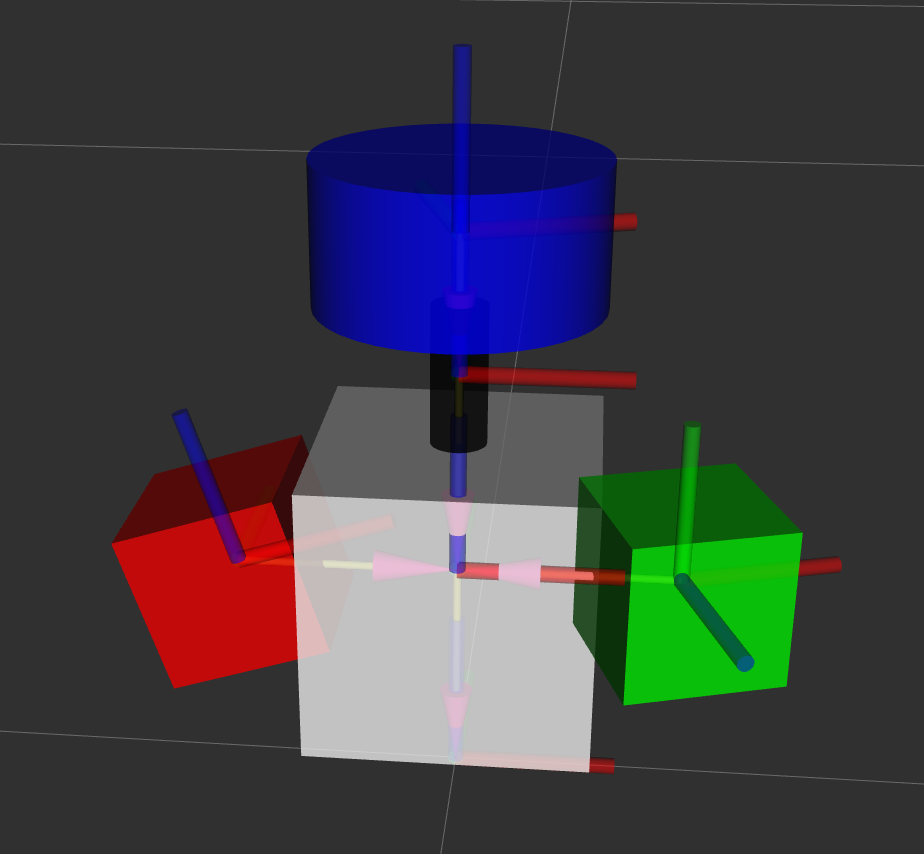
\includegraphics[width=0.23\linewidth]{img/simu2/model.png}
      \label{fig:simu2_model}
    }
    \subfigure[\normf{标定结果(正视图)}]{
      \centering
      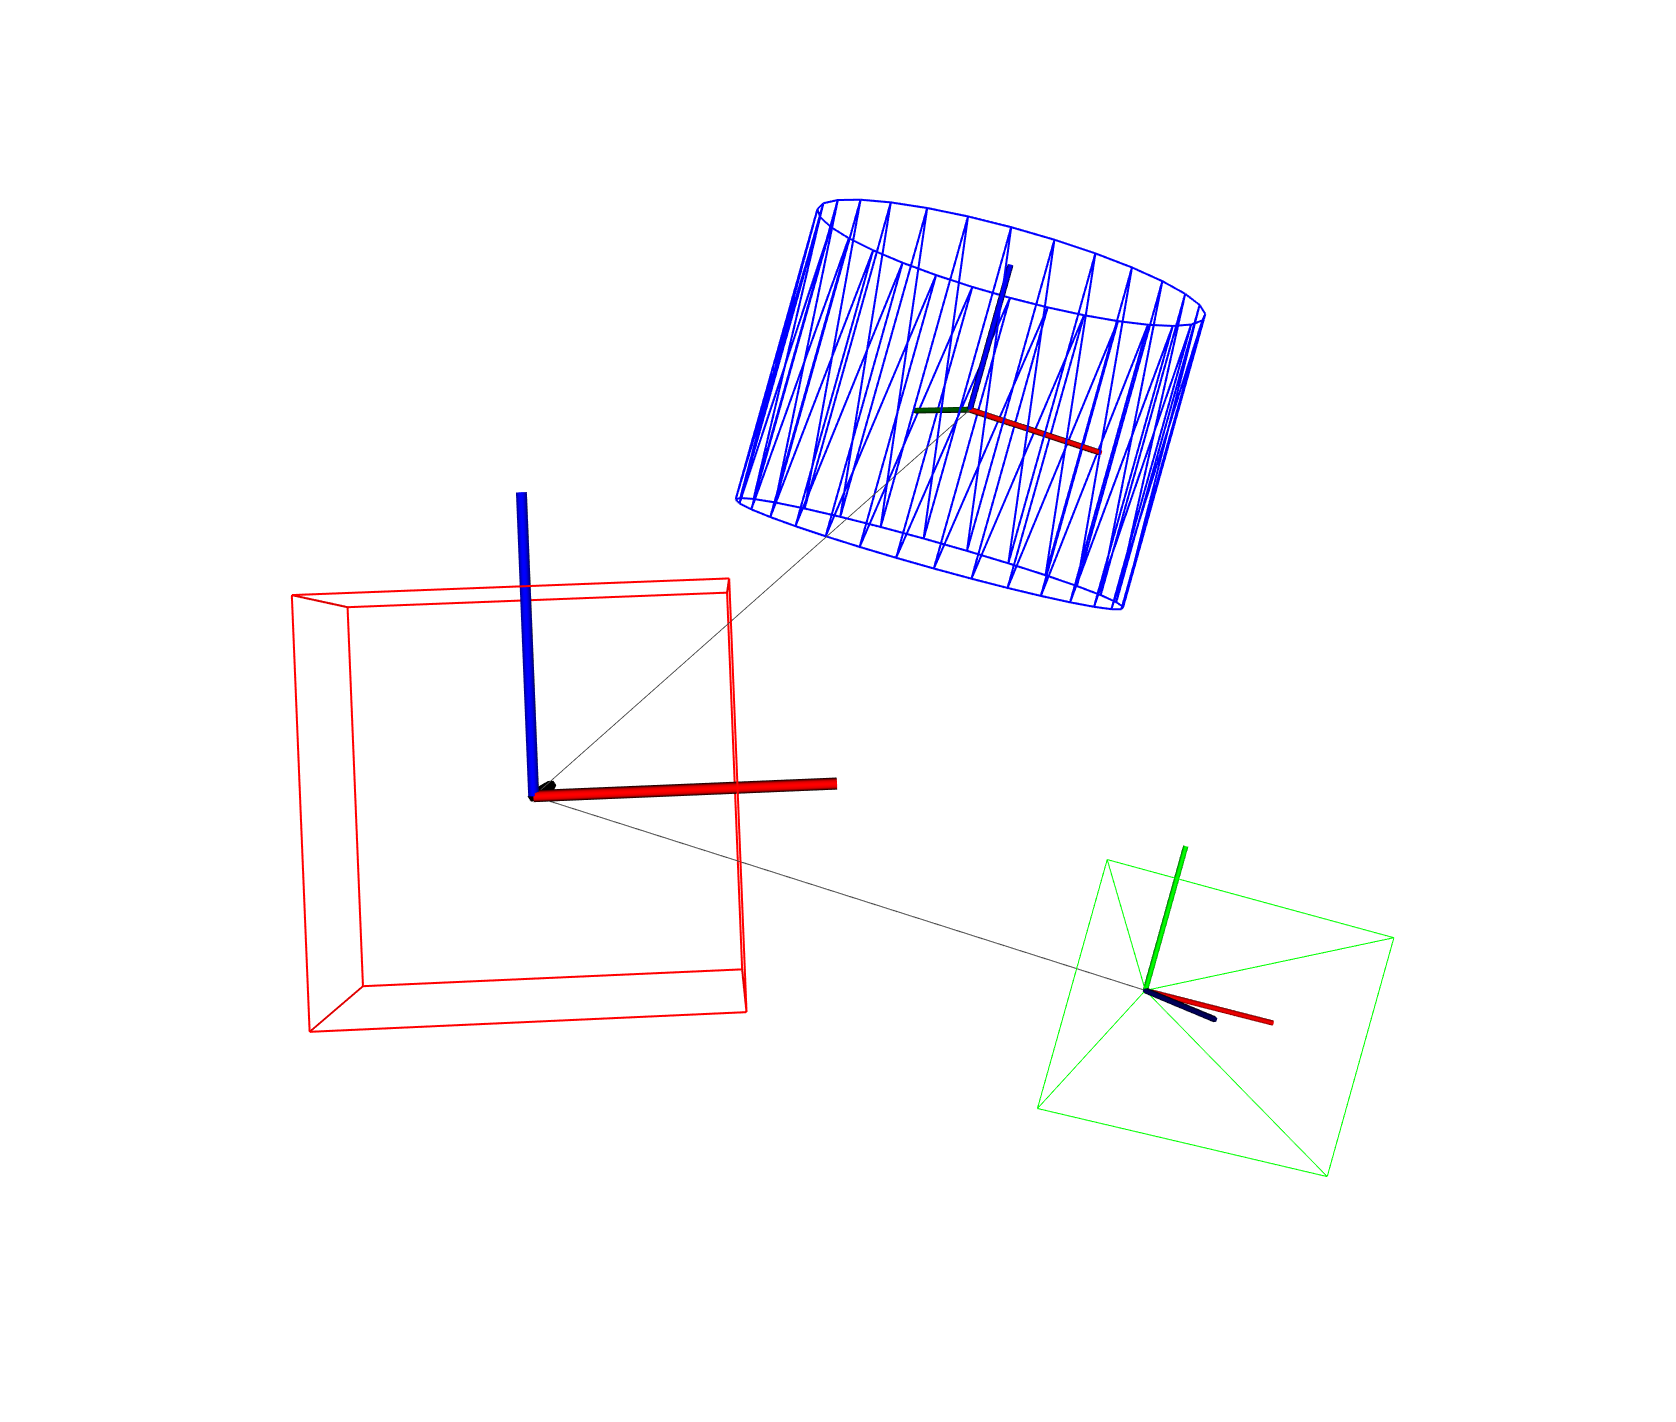
\includegraphics[width=0.23\linewidth]{img/simu2/calib_result1.png}
      \label{fig:simu2_calib_result1}
    }
    \subfigure[\normf{标定结果(俯视图)}]{
      \centering
      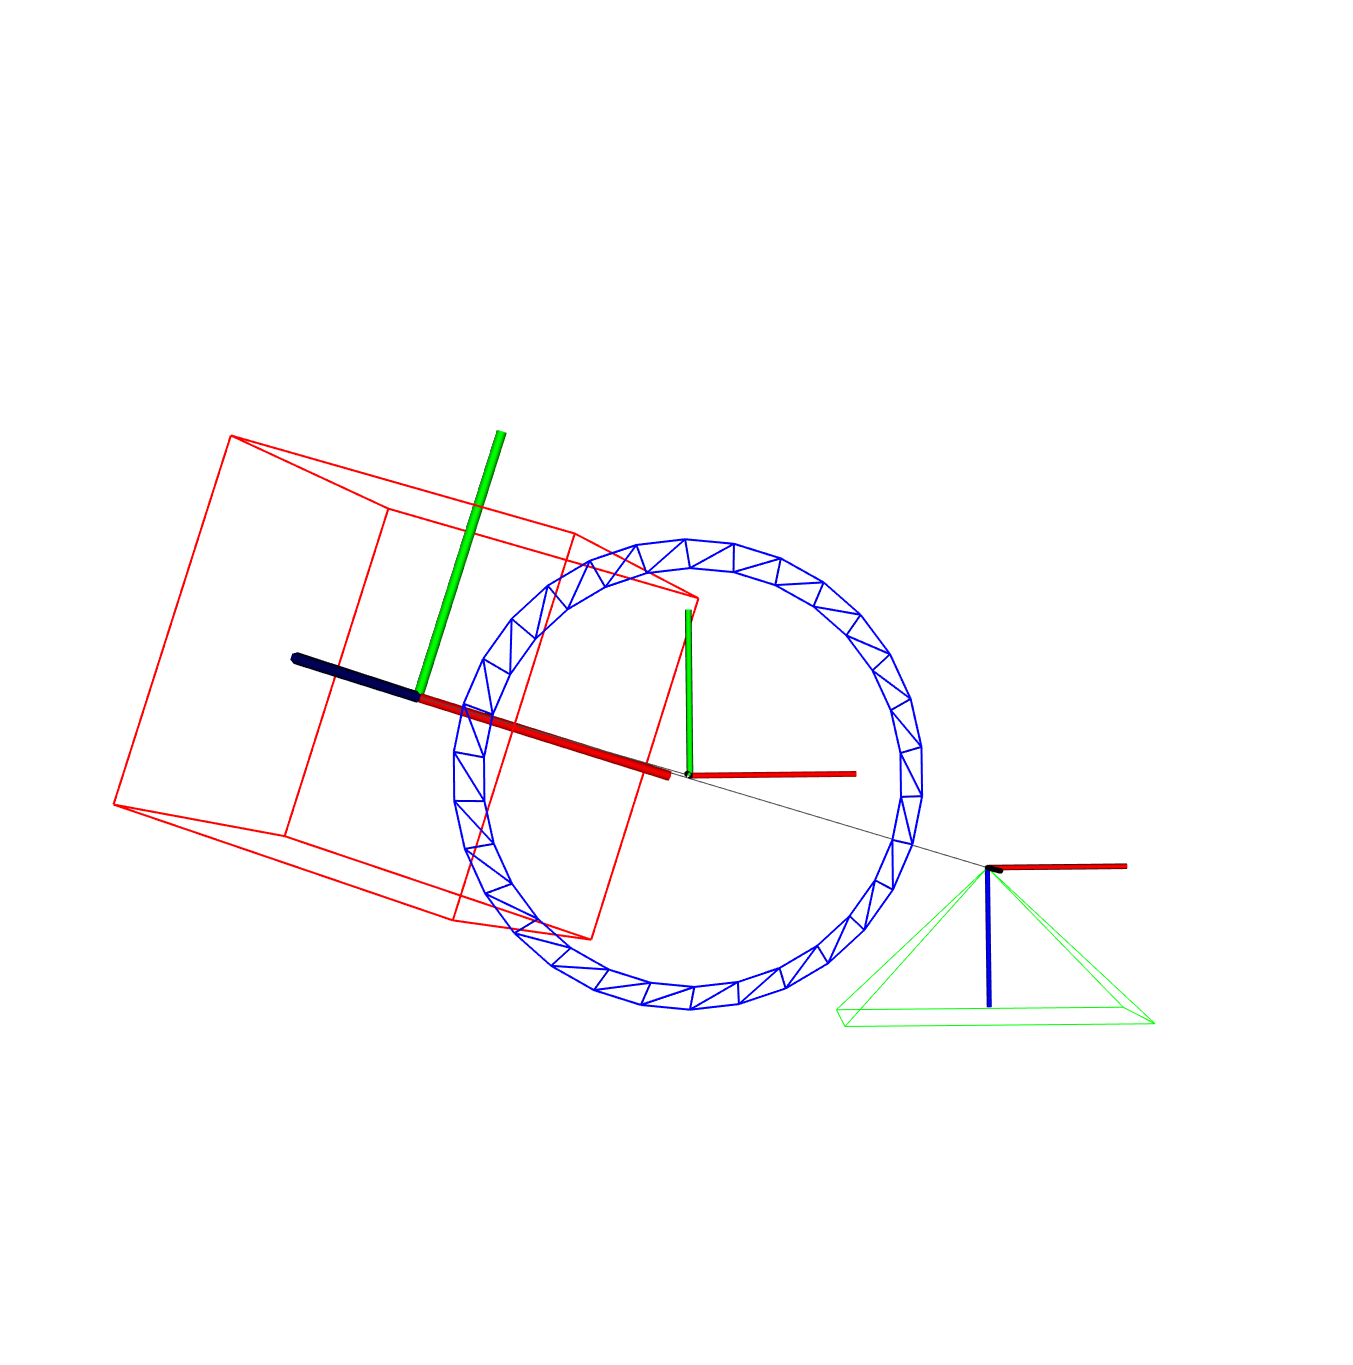
\includegraphics[width=0.23\linewidth]{img/simu2/calib_result2.png}
      \label{fig:simu2_calib_result2}
    }

    \caption{\normf{随机运动下系统可观性实验处理结果}}

    \label{fig:simu2_result}
  \end{figure}
}
%%%%%%%%%%%%%%%%%%%%%%%%%%%%%%%%%%%%%%%%%%%%%%%%%%%%%%%%%%%%%%%%%%%%%%%%%%%%%%%%%%%%%%%%%
\mlcomment{
  \begin{figure}[htbp]

    \centering
    \includegraphics[width=0.95\linewidth]{img/simu2/params_iter/abs_error.png}

    \caption{\normf{随机运动下系统可观性实验IMU/LiDAR/Camera外参和时延的收敛曲线}}
    \label{fig:simu2_evaluate}
  \end{figure}
}

为了直接通过法方程的数值表达形式来考察系统的可观性,在每次批处理迭代计算之前,我们基于Ceres的自动求导(Automatic Differentiation)功能,输出损失函数对相关参数的雅克比矩阵,而后构建出法方程中的矩阵$\boldsymbol{H}_{n\times n}$和向量$\boldsymbol{b}_{n\times 1}$。
以随机运动为例,所实现的标定系统的解算结果如图\ref{fig:simu2_result}所示\footnote{\normf{这里将所有待标定的参数都考虑进来,即包含了外参、时延参数及其他在可观性分析中没有考虑的其他参数。}},其中图\ref{fig:simu2_model}、\ref{fig:simu2_calib_result1}、\ref{fig:simu2_calib_result2}中红色传感器为IMU、绿色传感器为Camera、蓝色传感器为LiDAR。在三次批处理中,法方程$\boldsymbol{H}_{n\times n}\cdot\delta\boldsymbol{x}_{n\times 1}=\boldsymbol{b}_{n\times 1}$的数值表达如图\ref{fig:simu2_lm_equ}所示,其中:左侧方块为系数矩阵$\boldsymbol{H}_{n\times n}$,中间单列方块为参数向量的更新量$\delta\boldsymbol{x}_{n\times 1}$,且不同灰度表示不同的参数块(Parameter Block),右侧单列方块为向量$\boldsymbol{b}_{n\times 1}$;红色表示正值,蓝色表示负值,颜色越深,绝对值越大\footnote{\normf{为了更好的可视化,数值已通过函数$f(x)=x\cdot\vert x\vert^{-1}\cdot\log_{2}(\vert x\vert+1)$进行了映射。}},白色代表零值。

%%%%%%%%%%%%%%%%%%%%%%%%%%%%%%%%%%%%%%%%%%%%%%%%%%%%%%%%%%%%%%%%%%%%%%%%%%%%%%%%%%%%%%%%%
\mlcomment{
  \begin{figure}[h]
    \centering

    \subfigure[\normf{第一次迭代}]{
      \centering
      \begin{minipage}{0.62\linewidth}
        \centerline{\includegraphics[width=\textwidth]{img/simu2/system_oa/random/batch_opt_0.png}}
        \vspace{20pt}
      \end{minipage}
      \label{fig:simu2_lm_equ_0}
    }
    \subfigure[\normf{第二次(上)第三次(下)}]{
      \centering
      \begin{minipage}{0.25\linewidth}
        \vspace{20pt}
        \centerline{\includegraphics[width=\textwidth]{img/simu2/system_oa/random/batch_opt_1.png}}
        \vspace{22pt}
        \centerline{\includegraphics[width=\textwidth]{img/simu2/system_oa/random/batch_opt_2.png}}
        \vspace{35pt}
      \end{minipage}
      \label{fig:simu2_lm_equ_2_3}
    }
    \caption{\normf{随机运动下每次迭代时的法方程}}
    \label{fig:simu2_lm_equ}
  \end{figure}
}

为了更加直观的展示待求参数的可观性,我们通过等价行变换求解了法方程的行简化阶梯型。对于随机运动而言,其每次迭代时法方程的行简化阶梯型如图\ref{fig:simu2_lm_equ_echelon_form}所示。当参数$\delta\boldsymbol{x}(i)$可以被表示为其他参数的线性组合时,表示该参数不可观,反之则可观。注意到,使用该种方式考察参数可观性等价于使用系数矩阵的零空间$N(\boldsymbol{H})$进行参数可观性判断。
\mlcomment{
  \begin{figure}[h]
    \centering

    \subfigure[\normf{第一次}]{
      \centering
      \begin{minipage}{0.62\linewidth}
        \centerline{\includegraphics[width=\textwidth]{img/simu2/system_oa/random/echelon_form/batch_opt_0.png}}
        \vspace{20pt}
      \end{minipage}
      \label{fig:simu2_lm_equ_0_echelon_form}
    }
    \subfigure[\normf{第二次(上)第三次(下)}]{
      \centering
      \begin{minipage}{0.25\linewidth}
        \vspace{20pt}
        \centerline{\includegraphics[width=\textwidth]{img/simu2/system_oa/random/echelon_form/batch_opt_1.png}}
        \vspace{22pt}
        \centerline{\includegraphics[width=\textwidth]{img/simu2/system_oa/random/echelon_form/batch_opt_2.png}}
        \vspace{35pt}
      \end{minipage}
      \label{fig:simu2_lm_equ_2_3_echelon_form}
    }
    \caption{\normf{随机运动下每次批处理优化时法方程的行简化阶梯型}}
    \label{fig:simu2_lm_equ_echelon_form}
  \end{figure}
}

与模拟随机运动类似,通过修改模拟轨迹的函数表达,可以模拟不同类型的运动。基于模拟出的运动轨迹,在相同的仿真场景下进行传感器数据的采集并进行解算,最后可以得到类似于图\ref{fig:simu2_lm_equ}所示的实验结果。而后对其进行相应的分析,即可获得可观的参数及不可观的参数。

\subsection{\normf{系统可观性结论}}
基于上文的理论分析和实验验证可以得到,在通过自运动来标定多传感器参数时,不同的运动形式会对系统的可观性有着不同程度的影响。对于本文标定算法中外参和时参的估计而言,不同类型运动形式下的可观性结果如表\ref{tab:observability}所示。可以看到,在随机运动下,系统的外参和时参是可观的,与此相反的无运动形式下,整个系统是不可观的。
\begin{table*}[htbp]
  \centering
  \normf
  \begin{tabular}{l|ll}
    \hline
    {运动类型}     & {不可观}                                                             & {可观}                 \\ \hline
    {无运动}       & {外参、时参}                                                         & {-}                    \\
    {纯位移}       & {外参位移量}                                                         & {外参姿态量、时参}     \\
    {单轴旋转}     & {沿旋转轴${^{I}\boldsymbol{n}_{\boldsymbol{\phi}}}$方向的外参位移量} & {外参姿态量、时参}     \\
    {匀速圆周运动} & {时参、沿旋转轴${^{L\mid C}\boldsymbol{\omega}}$方向的外参姿态量}    & {外参位移量条件下可观} \\
    {随机运动}     & {-}                                                                  & {外参、时参}           \\
    \hline
  \end{tabular}
  \caption{\normf{不同运动形式下的系统外参和时延的可观性}}
  \label{tab:observability}
\end{table*}

基于系统可观性的测试结果可以得到,在使用本文提出的标定方法进行多传感器标定时,需要对载体进行充分的运动激励,并且针对性的避免上述运动类型中那些导致某些参数不可观的退化运动,以满足系统的可观性,保证参数估计的准确性。
